% **************************************************************************************************************
% A Classic Thesis Style
% An Homage to The Elements of Typographic Style
%
% Copyright (C) 2018 André Miede and Ivo Pletikosić
%
% If you like the style then I would appreciate a postcard. My address
% can be found in the file ClassicThesis.pdf. A collection of the
% postcards I received so far is available online at
% http://postcards.miede.de
%
% License:
% This program is free software; you can redistribute it and/or modify
% it under the terms of the GNU General Public License as published by
% the Free Software Foundation; either version 2 of the License, or
% (at your option) any later version.
%
% This program is distributed in the hope that it will be useful,
% but WITHOUT ANY WARRANTY; without even the implied warranty of
% MERCHANTABILITY or FITNESS FOR A PARTICULAR PURPOSE.  See the
% GNU General Public License for more details.
%
% You should have received a copy of the GNU General Public License
% along with this program; see the file COPYING.  If not, write to
% the Free Software Foundation, Inc., 59 Temple Place - Suite 330,
% Boston, MA 02111-1307, USA.
%
% PLEASE SEE ALSO THE AUTHORS' NOTE REGARDING THIS LICENSE
% IN THE DOCUMENTATION (ClassicThesis.pdf --> Chapter 1 / Chapter01.tex)
% **************************************************************************************************************
\RequirePackage{silence} % :-\
    \WarningFilter{scrreprt}{Usage of package `titlesec'}
    %\WarningFilter{scrreprt}{Activating an ugly workaround}
    \WarningFilter{titlesec}{Non standard sectioning command detected}
\documentclass[ twoside,openright,titlepage,numbers=noenddot,%1headlines,
                headinclude,footinclude,cleardoublepage=empty,abstract=on,
                BCOR=5mm,paper=a4,fontsize=11pt
                ]{scrreprt}

%********************************************************************
% Note: Make all your adjustments in here
%*******************************************************
% ****************************************************************************************************
% classicthesis-config.tex
% formerly known as loadpackages.sty, classicthesis-ldpkg.sty, and classicthesis-preamble.sty
% Use it at the beginning of your ClassicThesis.tex, or as a LaTeX Preamble
% in your ClassicThesis.{tex,lyx} with % ****************************************************************************************************
% classicthesis-config.tex
% formerly known as loadpackages.sty, classicthesis-ldpkg.sty, and classicthesis-preamble.sty
% Use it at the beginning of your ClassicThesis.tex, or as a LaTeX Preamble
% in your ClassicThesis.{tex,lyx} with % ****************************************************************************************************
% classicthesis-config.tex
% formerly known as loadpackages.sty, classicthesis-ldpkg.sty, and classicthesis-preamble.sty
% Use it at the beginning of your ClassicThesis.tex, or as a LaTeX Preamble
% in your ClassicThesis.{tex,lyx} with \input{classicthesis-config}
% ****************************************************************************************************
% If you like the classicthesis, then I would appreciate a postcard.
% My address can be found in the file ClassicThesis.pdf. A collection
% of the postcards I received so far is available online at
% http://postcards.miede.de
% ****************************************************************************************************


% ****************************************************************************************************
% 0. Set the encoding of your files. UTF-8 is the only sensible encoding nowadays. If you can't read
% äöüßáéçèê∂åëæƒÏ€ then change the encoding setting in your editor, not the line below. If your editor
% does not support utf8 use another editor!
% ****************************************************************************************************
\PassOptionsToPackage{utf8}{inputenc}
  \usepackage{inputenc}

\PassOptionsToPackage{T1}{fontenc} % T2A for cyrillics
  \usepackage{fontenc}


% ****************************************************************************************************
% 1. Configure classicthesis for your needs here, e.g., remove "drafting" below
% in order to deactivate the time-stamp on the pages
% (see ClassicThesis.pdf for more information):
% ****************************************************************************************************
\PassOptionsToPackage{
  drafting=true,    % print version information on the bottom of the pages
  tocaligned=false, % the left column of the toc will be aligned (no indentation)
  dottedtoc=false,  % page numbers in ToC flushed right
  eulerchapternumbers=true, % use AMS Euler for chapter font (otherwise Palatino)
  linedheaders=false,       % chaper headers will have line above and beneath
  floatperchapter=true,     % numbering per chapter for all floats (i.e., Figure 1.1)
  eulermath=false,  % use awesome Euler fonts for mathematical formulae (only with pdfLaTeX)
  beramono=true,    % toggle a nice monospaced font (w/ bold)
  palatino=true,    % deactivate standard font for loading another one, see the last section at the end of this file for suggestions
  style=classicthesis % classicthesis, arsclassica
}{classicthesis}


% ****************************************************************************************************
% 2. Personal data and user ad-hoc commands (insert your own data here)
% ****************************************************************************************************
\newcommand{\myTitle}{Generalización de Meta-programas con Tipado Dependiente en Mtac2\xspace}
\newcommand{\mySubtitle}{Un desarrollo de generalización cuasi automática de meta-programas\xspace}
\newcommand{\myDegree}{Licenciado en Ciencias de la Computación\xspace}
\newcommand{\myName}{Ignacio Tiraboschi\xspace}
\newcommand{\myProf}{Put name here\xspace}
\newcommand{\myOtherProf}{Put name here\xspace}
\newcommand{\mySupervisor}{Dr. Beta Ziliani\xspace}
\newcommand{\myFaculty}{FAMAF\xspace}
\newcommand{\myDepartment}{Put data here\xspace}
\newcommand{\myUni}{Universidad Nacional de Córdoba\xspace}
\newcommand{\myLocation}{Córdoba\xspace}
\newcommand{\myTime}{Marzo 2020\xspace}
\newcommand{\myVersion}{\classicthesis}

% ********************************************************************
% Setup, finetuning, and useful commands
% ********************************************************************
\providecommand{\mLyX}{L\kern-.1667em\lower.25em\hbox{Y}\kern-.125emX\@}
\newcommand{\ie}{i.\,e.}
\newcommand{\Ie}{I.\,e.}
\newcommand{\eg}{e.\,g.}
\newcommand{\Eg}{E.\,g.}
\newcommand{\code}[1]{\texttt{#1}}
\newcommand{\nat}{\mathbb{N}}
\newcommand{\lift}{{\scshape Lift}}
% ****************************************************************************************************


% ****************************************************************************************************
% 3. Loading some handy packages
% ****************************************************************************************************
% ********************************************************************
% Packages with options that might require adjustments
% ********************************************************************
\PassOptionsToPackage{spanish,es-lcroman}{babel} % change this to your language(s), main language last
% Spanish languages need extra options in order to work with this template
%\PassOptionsToPackage{spanish,es-lcroman}{babel}
    \usepackage{babel}

\usepackage{csquotes}
\PassOptionsToPackage{%
  %backend=biber,bibencoding=utf8, %instead of bibtex
  backend=bibtex8,bibencoding=ascii,%
  language=auto,%
  style=numeric-comp,%
  %style=authoryear-comp, % Author 1999, 2010
  %bibstyle=authoryear,dashed=false, % dashed: substitute rep. author with ---
  sorting=nyt, % name, year, title
  maxbibnames=10, % default: 3, et al.
  %backref=true,%
  natbib=true % natbib compatibility mode (\citep and \citet still work)
}{biblatex}
    \usepackage{biblatex}

\PassOptionsToPackage{fleqn}{amsmath}       % math environments and more by the AMS
  \usepackage{amsmath}

% ********************************************************************
% General useful packages
% ********************************************************************
\usepackage{graphicx} %
\usepackage{scrhack} % fix warnings when using KOMA with listings package
\usepackage{xspace} % to get the spacing after macros right
\PassOptionsToPackage{printonlyused,smaller}{acronym}
  \usepackage{acronym} % nice macros for handling all acronyms in the thesis
  %\renewcommand{\bflabel}[1]{{#1}\hfill} % fix the list of acronyms --> no longer working
  %\renewcommand*{\acsfont}[1]{\textsc{#1}}
  %\renewcommand*{\aclabelfont}[1]{\acsfont{#1}}
  %\def\bflabel#1{{#1\hfill}}
  \def\bflabel#1{{\acsfont{#1}\hfill}}
  \def\aclabelfont#1{\acsfont{#1}}
\usepackage{amsthm}
\theoremstyle{definition}
\newtheorem{exmp}{Ejemplo}[section]
% ****************************************************************************************************
%\usepackage{pgfplots} % External TikZ/PGF support (thanks to Andreas Nautsch)
%\usetikzlibrary{external}
%\tikzexternalize[mode=list and make, prefix=ext-tikz/]
% ****************************************************************************************************


% ****************************************************************************************************
% 4. Setup floats: tables, (sub)figures, and captions
% ****************************************************************************************************
\usepackage{tabularx} % better tables
  \setlength{\extrarowheight}{3pt} % increase table row height
\newcommand{\tableheadline}[1]{\multicolumn{1}{l}{\spacedlowsmallcaps{#1}}}
\newcommand{\myfloatalign}{\centering} % to be used with each float for alignment
\usepackage{subfig}
% ****************************************************************************************************


% ****************************************************************************************************
% 5. Setup code listings
% ****************************************************************************************************
% \usepackage{listings}
\usepackage{listings,lstlangcoq,bold-extra}
\lstset{basicstyle=\ttfamily,language=Coq,showstringspaces=false}
%\lstset{emph={trueIndex,root},emphstyle=\color{BlueViolet}}%\underbar} % for special keywords
\lstset{language=Coq,
  morekeywords={PassOptionsToPackage,selectlanguage},
  keywordstyle=\color{RoyalBlue},%\bfseries,
  basicstyle=\small\ttfamily,
  %identifierstyle=\color{NavyBlue},
  commentstyle=\color{Green}\ttfamily,
  stringstyle=\rmfamily,
  numbers=none,%left,%
  numberstyle=\scriptsize,%\tiny
  stepnumber=5,
  numbersep=8pt,
  showstringspaces=false,
  breaklines=true,
  %frameround=ftff,
  %frame=single,
  belowcaptionskip=.75\baselineskip
  %frame=L
}
% ****************************************************************************************************




% ****************************************************************************************************
% 6. Last calls before the bar closes
% ****************************************************************************************************
% ********************************************************************
% Her Majesty herself
% ********************************************************************
\usepackage{classicthesis}


% ********************************************************************
% Fine-tune hyperreferences (hyperref should be called last)
% ********************************************************************
\hypersetup{%
  %draft, % hyperref's draft mode, for printing see below
  colorlinks=true, linktocpage=true, pdfstartpage=3, pdfstartview=FitV,%
  % uncomment the following line if you want to have black links (e.g., for printing)
  %colorlinks=false, linktocpage=false, pdfstartpage=3, pdfstartview=FitV, pdfborder={0 0 0},%
  breaklinks=true, pageanchor=true,%
  pdfpagemode=UseNone, %
  % pdfpagemode=UseOutlines,%
  plainpages=false, bookmarksnumbered, bookmarksopen=true, bookmarksopenlevel=1,%
  hypertexnames=true, pdfhighlight=/O,%nesting=true,%frenchlinks,%
  urlcolor=CTurl, linkcolor=CTlink, citecolor=CTcitation, %pagecolor=RoyalBlue,%
  %urlcolor=Black, linkcolor=Black, citecolor=Black, %pagecolor=Black,%
  pdftitle={\myTitle},%
  pdfauthor={\textcopyright\ \myName, \myUni, \myFaculty},%
  pdfsubject={},%
  pdfkeywords={},%
  pdfcreator={pdfLaTeX},%
  pdfproducer={LaTeX with hyperref and classicthesis}%
}


% ********************************************************************
% Setup autoreferences (hyperref and babel)
% ********************************************************************
% There are some issues regarding autorefnames
% http://www.tex.ac.uk/cgi-bin/texfaq2html?label=latexwords
% you have to redefine the macros for the
% language you use, e.g., american, ngerman
% (as chosen when loading babel/AtBeginDocument)
% ********************************************************************
\makeatletter
\@ifpackageloaded{babel}%
  {%
    \addto\extrasamerican{%
      \renewcommand*{\figureautorefname}{Figure}%
      \renewcommand*{\tableautorefname}{Table}%
      \renewcommand*{\partautorefname}{Part}%
      \renewcommand*{\chapterautorefname}{Chapter}%
      \renewcommand*{\sectionautorefname}{Section}%
      \renewcommand*{\subsectionautorefname}{Section}%
      \renewcommand*{\subsubsectionautorefname}{Section}%
    }%
    \addto\extrasngerman{%
      \renewcommand*{\paragraphautorefname}{Absatz}%
      \renewcommand*{\subparagraphautorefname}{Unterabsatz}%
      \renewcommand*{\footnoteautorefname}{Fu\"snote}%
      \renewcommand*{\FancyVerbLineautorefname}{Zeile}%
      \renewcommand*{\theoremautorefname}{Theorem}%
      \renewcommand*{\appendixautorefname}{Anhang}%
      \renewcommand*{\equationautorefname}{Gleichung}%
      \renewcommand*{\itemautorefname}{Punkt}%
    }%
      % Fix to getting autorefs for subfigures right (thanks to Belinda Vogt for changing the definition)
      \providecommand{\subfigureautorefname}{\figureautorefname}%
    }{\relax}
\makeatother


% ********************************************************************
% Development Stuff
% ********************************************************************
\listfiles
%\PassOptionsToPackage{l2tabu,orthodox,abort}{nag}
%  \usepackage{nag}
%\PassOptionsToPackage{warning, all}{onlyamsmath}
%  \usepackage{onlyamsmath}


% ****************************************************************************************************
% 7. Further adjustments (experimental)
% ****************************************************************************************************
% ********************************************************************
% Changing the text area
% ********************************************************************
%\areaset[current]{312pt}{761pt} % 686 (factor 2.2) + 33 head + 42 head \the\footskip
%\setlength{\marginparwidth}{7em}%
%\setlength{\marginparsep}{2em}%

% ********************************************************************
% Using different fonts
% ********************************************************************
%\usepackage[oldstylenums]{kpfonts} % oldstyle notextcomp
% \usepackage[osf]{libertine}
%\usepackage[light,condensed,math]{iwona}
%\renewcommand{\sfdefault}{iwona}
%\usepackage{lmodern} % <-- no osf support :-(
%\usepackage{cfr-lm} %
%\usepackage[urw-garamond]{mathdesign} <-- no osf support :-(
%\usepackage[default,osfigures]{opensans} % scale=0.95
%\usepackage[sfdefault]{FiraSans}
% \usepackage[opticals,mathlf]{MinionPro} % onlytext
% ********************************************************************
%\usepackage[largesc,osf]{newpxtext}
%\linespread{1.05} % a bit more for Palatino
% Used to fix these:
% https://bitbucket.org/amiede/classicthesis/issues/139/italics-in-pallatino-capitals-chapter
% https://bitbucket.org/amiede/classicthesis/issues/45/problema-testatine-su-classicthesis-style
% ********************************************************************
% ****************************************************************************************************

% ****************************************************************************************************
% If you like the classicthesis, then I would appreciate a postcard.
% My address can be found in the file ClassicThesis.pdf. A collection
% of the postcards I received so far is available online at
% http://postcards.miede.de
% ****************************************************************************************************


% ****************************************************************************************************
% 0. Set the encoding of your files. UTF-8 is the only sensible encoding nowadays. If you can't read
% äöüßáéçèê∂åëæƒÏ€ then change the encoding setting in your editor, not the line below. If your editor
% does not support utf8 use another editor!
% ****************************************************************************************************
\PassOptionsToPackage{utf8}{inputenc}
  \usepackage{inputenc}

\PassOptionsToPackage{T1}{fontenc} % T2A for cyrillics
  \usepackage{fontenc}


% ****************************************************************************************************
% 1. Configure classicthesis for your needs here, e.g., remove "drafting" below
% in order to deactivate the time-stamp on the pages
% (see ClassicThesis.pdf for more information):
% ****************************************************************************************************
\PassOptionsToPackage{
  drafting=true,    % print version information on the bottom of the pages
  tocaligned=false, % the left column of the toc will be aligned (no indentation)
  dottedtoc=false,  % page numbers in ToC flushed right
  eulerchapternumbers=true, % use AMS Euler for chapter font (otherwise Palatino)
  linedheaders=false,       % chaper headers will have line above and beneath
  floatperchapter=true,     % numbering per chapter for all floats (i.e., Figure 1.1)
  eulermath=false,  % use awesome Euler fonts for mathematical formulae (only with pdfLaTeX)
  beramono=true,    % toggle a nice monospaced font (w/ bold)
  palatino=true,    % deactivate standard font for loading another one, see the last section at the end of this file for suggestions
  style=classicthesis % classicthesis, arsclassica
}{classicthesis}


% ****************************************************************************************************
% 2. Personal data and user ad-hoc commands (insert your own data here)
% ****************************************************************************************************
\newcommand{\myTitle}{Generalización de Meta-programas con Tipado Dependiente en Mtac2\xspace}
\newcommand{\mySubtitle}{Un desarrollo de generalización cuasi automática de meta-programas\xspace}
\newcommand{\myDegree}{Licenciado en Ciencias de la Computación\xspace}
\newcommand{\myName}{Ignacio Tiraboschi\xspace}
\newcommand{\myProf}{Put name here\xspace}
\newcommand{\myOtherProf}{Put name here\xspace}
\newcommand{\mySupervisor}{Dr. Beta Ziliani\xspace}
\newcommand{\myFaculty}{FAMAF\xspace}
\newcommand{\myDepartment}{Put data here\xspace}
\newcommand{\myUni}{Universidad Nacional de Córdoba\xspace}
\newcommand{\myLocation}{Córdoba\xspace}
\newcommand{\myTime}{Marzo 2020\xspace}
\newcommand{\myVersion}{\classicthesis}

% ********************************************************************
% Setup, finetuning, and useful commands
% ********************************************************************
\providecommand{\mLyX}{L\kern-.1667em\lower.25em\hbox{Y}\kern-.125emX\@}
\newcommand{\ie}{i.\,e.}
\newcommand{\Ie}{I.\,e.}
\newcommand{\eg}{e.\,g.}
\newcommand{\Eg}{E.\,g.}
\newcommand{\code}[1]{\texttt{#1}}
\newcommand{\nat}{\mathbb{N}}
\newcommand{\lift}{{\scshape Lift}}
% ****************************************************************************************************


% ****************************************************************************************************
% 3. Loading some handy packages
% ****************************************************************************************************
% ********************************************************************
% Packages with options that might require adjustments
% ********************************************************************
\PassOptionsToPackage{spanish,es-lcroman}{babel} % change this to your language(s), main language last
% Spanish languages need extra options in order to work with this template
%\PassOptionsToPackage{spanish,es-lcroman}{babel}
    \usepackage{babel}

\usepackage{csquotes}
\PassOptionsToPackage{%
  %backend=biber,bibencoding=utf8, %instead of bibtex
  backend=bibtex8,bibencoding=ascii,%
  language=auto,%
  style=numeric-comp,%
  %style=authoryear-comp, % Author 1999, 2010
  %bibstyle=authoryear,dashed=false, % dashed: substitute rep. author with ---
  sorting=nyt, % name, year, title
  maxbibnames=10, % default: 3, et al.
  %backref=true,%
  natbib=true % natbib compatibility mode (\citep and \citet still work)
}{biblatex}
    \usepackage{biblatex}

\PassOptionsToPackage{fleqn}{amsmath}       % math environments and more by the AMS
  \usepackage{amsmath}

% ********************************************************************
% General useful packages
% ********************************************************************
\usepackage{graphicx} %
\usepackage{scrhack} % fix warnings when using KOMA with listings package
\usepackage{xspace} % to get the spacing after macros right
\PassOptionsToPackage{printonlyused,smaller}{acronym}
  \usepackage{acronym} % nice macros for handling all acronyms in the thesis
  %\renewcommand{\bflabel}[1]{{#1}\hfill} % fix the list of acronyms --> no longer working
  %\renewcommand*{\acsfont}[1]{\textsc{#1}}
  %\renewcommand*{\aclabelfont}[1]{\acsfont{#1}}
  %\def\bflabel#1{{#1\hfill}}
  \def\bflabel#1{{\acsfont{#1}\hfill}}
  \def\aclabelfont#1{\acsfont{#1}}
\usepackage{amsthm}
\theoremstyle{definition}
\newtheorem{exmp}{Ejemplo}[section]
% ****************************************************************************************************
%\usepackage{pgfplots} % External TikZ/PGF support (thanks to Andreas Nautsch)
%\usetikzlibrary{external}
%\tikzexternalize[mode=list and make, prefix=ext-tikz/]
% ****************************************************************************************************


% ****************************************************************************************************
% 4. Setup floats: tables, (sub)figures, and captions
% ****************************************************************************************************
\usepackage{tabularx} % better tables
  \setlength{\extrarowheight}{3pt} % increase table row height
\newcommand{\tableheadline}[1]{\multicolumn{1}{l}{\spacedlowsmallcaps{#1}}}
\newcommand{\myfloatalign}{\centering} % to be used with each float for alignment
\usepackage{subfig}
% ****************************************************************************************************


% ****************************************************************************************************
% 5. Setup code listings
% ****************************************************************************************************
% \usepackage{listings}
\usepackage{listings,lstlangcoq,bold-extra}
\lstset{basicstyle=\ttfamily,language=Coq,showstringspaces=false}
%\lstset{emph={trueIndex,root},emphstyle=\color{BlueViolet}}%\underbar} % for special keywords
\lstset{language=Coq,
  morekeywords={PassOptionsToPackage,selectlanguage},
  keywordstyle=\color{RoyalBlue},%\bfseries,
  basicstyle=\small\ttfamily,
  %identifierstyle=\color{NavyBlue},
  commentstyle=\color{Green}\ttfamily,
  stringstyle=\rmfamily,
  numbers=none,%left,%
  numberstyle=\scriptsize,%\tiny
  stepnumber=5,
  numbersep=8pt,
  showstringspaces=false,
  breaklines=true,
  %frameround=ftff,
  %frame=single,
  belowcaptionskip=.75\baselineskip
  %frame=L
}
% ****************************************************************************************************




% ****************************************************************************************************
% 6. Last calls before the bar closes
% ****************************************************************************************************
% ********************************************************************
% Her Majesty herself
% ********************************************************************
\usepackage{classicthesis}


% ********************************************************************
% Fine-tune hyperreferences (hyperref should be called last)
% ********************************************************************
\hypersetup{%
  %draft, % hyperref's draft mode, for printing see below
  colorlinks=true, linktocpage=true, pdfstartpage=3, pdfstartview=FitV,%
  % uncomment the following line if you want to have black links (e.g., for printing)
  %colorlinks=false, linktocpage=false, pdfstartpage=3, pdfstartview=FitV, pdfborder={0 0 0},%
  breaklinks=true, pageanchor=true,%
  pdfpagemode=UseNone, %
  % pdfpagemode=UseOutlines,%
  plainpages=false, bookmarksnumbered, bookmarksopen=true, bookmarksopenlevel=1,%
  hypertexnames=true, pdfhighlight=/O,%nesting=true,%frenchlinks,%
  urlcolor=CTurl, linkcolor=CTlink, citecolor=CTcitation, %pagecolor=RoyalBlue,%
  %urlcolor=Black, linkcolor=Black, citecolor=Black, %pagecolor=Black,%
  pdftitle={\myTitle},%
  pdfauthor={\textcopyright\ \myName, \myUni, \myFaculty},%
  pdfsubject={},%
  pdfkeywords={},%
  pdfcreator={pdfLaTeX},%
  pdfproducer={LaTeX with hyperref and classicthesis}%
}


% ********************************************************************
% Setup autoreferences (hyperref and babel)
% ********************************************************************
% There are some issues regarding autorefnames
% http://www.tex.ac.uk/cgi-bin/texfaq2html?label=latexwords
% you have to redefine the macros for the
% language you use, e.g., american, ngerman
% (as chosen when loading babel/AtBeginDocument)
% ********************************************************************
\makeatletter
\@ifpackageloaded{babel}%
  {%
    \addto\extrasamerican{%
      \renewcommand*{\figureautorefname}{Figure}%
      \renewcommand*{\tableautorefname}{Table}%
      \renewcommand*{\partautorefname}{Part}%
      \renewcommand*{\chapterautorefname}{Chapter}%
      \renewcommand*{\sectionautorefname}{Section}%
      \renewcommand*{\subsectionautorefname}{Section}%
      \renewcommand*{\subsubsectionautorefname}{Section}%
    }%
    \addto\extrasngerman{%
      \renewcommand*{\paragraphautorefname}{Absatz}%
      \renewcommand*{\subparagraphautorefname}{Unterabsatz}%
      \renewcommand*{\footnoteautorefname}{Fu\"snote}%
      \renewcommand*{\FancyVerbLineautorefname}{Zeile}%
      \renewcommand*{\theoremautorefname}{Theorem}%
      \renewcommand*{\appendixautorefname}{Anhang}%
      \renewcommand*{\equationautorefname}{Gleichung}%
      \renewcommand*{\itemautorefname}{Punkt}%
    }%
      % Fix to getting autorefs for subfigures right (thanks to Belinda Vogt for changing the definition)
      \providecommand{\subfigureautorefname}{\figureautorefname}%
    }{\relax}
\makeatother


% ********************************************************************
% Development Stuff
% ********************************************************************
\listfiles
%\PassOptionsToPackage{l2tabu,orthodox,abort}{nag}
%  \usepackage{nag}
%\PassOptionsToPackage{warning, all}{onlyamsmath}
%  \usepackage{onlyamsmath}


% ****************************************************************************************************
% 7. Further adjustments (experimental)
% ****************************************************************************************************
% ********************************************************************
% Changing the text area
% ********************************************************************
%\areaset[current]{312pt}{761pt} % 686 (factor 2.2) + 33 head + 42 head \the\footskip
%\setlength{\marginparwidth}{7em}%
%\setlength{\marginparsep}{2em}%

% ********************************************************************
% Using different fonts
% ********************************************************************
%\usepackage[oldstylenums]{kpfonts} % oldstyle notextcomp
% \usepackage[osf]{libertine}
%\usepackage[light,condensed,math]{iwona}
%\renewcommand{\sfdefault}{iwona}
%\usepackage{lmodern} % <-- no osf support :-(
%\usepackage{cfr-lm} %
%\usepackage[urw-garamond]{mathdesign} <-- no osf support :-(
%\usepackage[default,osfigures]{opensans} % scale=0.95
%\usepackage[sfdefault]{FiraSans}
% \usepackage[opticals,mathlf]{MinionPro} % onlytext
% ********************************************************************
%\usepackage[largesc,osf]{newpxtext}
%\linespread{1.05} % a bit more for Palatino
% Used to fix these:
% https://bitbucket.org/amiede/classicthesis/issues/139/italics-in-pallatino-capitals-chapter
% https://bitbucket.org/amiede/classicthesis/issues/45/problema-testatine-su-classicthesis-style
% ********************************************************************
% ****************************************************************************************************

% ****************************************************************************************************
% If you like the classicthesis, then I would appreciate a postcard.
% My address can be found in the file ClassicThesis.pdf. A collection
% of the postcards I received so far is available online at
% http://postcards.miede.de
% ****************************************************************************************************


% ****************************************************************************************************
% 0. Set the encoding of your files. UTF-8 is the only sensible encoding nowadays. If you can't read
% äöüßáéçèê∂åëæƒÏ€ then change the encoding setting in your editor, not the line below. If your editor
% does not support utf8 use another editor!
% ****************************************************************************************************
\PassOptionsToPackage{utf8}{inputenc}
  \usepackage{inputenc}

\PassOptionsToPackage{T1}{fontenc} % T2A for cyrillics
  \usepackage{fontenc}


% ****************************************************************************************************
% 1. Configure classicthesis for your needs here, e.g., remove "drafting" below
% in order to deactivate the time-stamp on the pages
% (see ClassicThesis.pdf for more information):
% ****************************************************************************************************
\PassOptionsToPackage{
  drafting=true,    % print version information on the bottom of the pages
  tocaligned=false, % the left column of the toc will be aligned (no indentation)
  dottedtoc=false,  % page numbers in ToC flushed right
  eulerchapternumbers=true, % use AMS Euler for chapter font (otherwise Palatino)
  linedheaders=false,       % chaper headers will have line above and beneath
  floatperchapter=true,     % numbering per chapter for all floats (i.e., Figure 1.1)
  eulermath=false,  % use awesome Euler fonts for mathematical formulae (only with pdfLaTeX)
  beramono=true,    % toggle a nice monospaced font (w/ bold)
  palatino=true,    % deactivate standard font for loading another one, see the last section at the end of this file for suggestions
  style=classicthesis % classicthesis, arsclassica
}{classicthesis}


% ****************************************************************************************************
% 2. Personal data and user ad-hoc commands (insert your own data here)
% ****************************************************************************************************
\newcommand{\myTitle}{Generalización de Meta-programas con Tipado Dependiente en Mtac2\xspace}
\newcommand{\mySubtitle}{Un desarrollo de generalización cuasi automática de meta-programas\xspace}
\newcommand{\myDegree}{Licenciado en Ciencias de la Computación\xspace}
\newcommand{\myName}{Ignacio Tiraboschi\xspace}
\newcommand{\myProf}{Put name here\xspace}
\newcommand{\myOtherProf}{Put name here\xspace}
\newcommand{\mySupervisor}{Dr. Beta Ziliani\xspace}
\newcommand{\myFaculty}{FAMAF\xspace}
\newcommand{\myDepartment}{Put data here\xspace}
\newcommand{\myUni}{Universidad Nacional de Córdoba\xspace}
\newcommand{\myLocation}{Córdoba\xspace}
\newcommand{\myTime}{Marzo 2020\xspace}
\newcommand{\myVersion}{\classicthesis}

% ********************************************************************
% Setup, finetuning, and useful commands
% ********************************************************************
\providecommand{\mLyX}{L\kern-.1667em\lower.25em\hbox{Y}\kern-.125emX\@}
\newcommand{\ie}{i.\,e.}
\newcommand{\Ie}{I.\,e.}
\newcommand{\eg}{e.\,g.}
\newcommand{\Eg}{E.\,g.}
\newcommand{\code}[1]{\texttt{#1}}
\newcommand{\nat}{\mathbb{N}}
\newcommand{\lift}{{\scshape Lift}}
% ****************************************************************************************************


% ****************************************************************************************************
% 3. Loading some handy packages
% ****************************************************************************************************
% ********************************************************************
% Packages with options that might require adjustments
% ********************************************************************
\PassOptionsToPackage{spanish,es-lcroman}{babel} % change this to your language(s), main language last
% Spanish languages need extra options in order to work with this template
%\PassOptionsToPackage{spanish,es-lcroman}{babel}
    \usepackage{babel}

\usepackage{csquotes}
\PassOptionsToPackage{%
  %backend=biber,bibencoding=utf8, %instead of bibtex
  backend=bibtex8,bibencoding=ascii,%
  language=auto,%
  style=numeric-comp,%
  %style=authoryear-comp, % Author 1999, 2010
  %bibstyle=authoryear,dashed=false, % dashed: substitute rep. author with ---
  sorting=nyt, % name, year, title
  maxbibnames=10, % default: 3, et al.
  %backref=true,%
  natbib=true % natbib compatibility mode (\citep and \citet still work)
}{biblatex}
    \usepackage{biblatex}

\PassOptionsToPackage{fleqn}{amsmath}       % math environments and more by the AMS
  \usepackage{amsmath}

% ********************************************************************
% General useful packages
% ********************************************************************
\usepackage{graphicx} %
\usepackage{scrhack} % fix warnings when using KOMA with listings package
\usepackage{xspace} % to get the spacing after macros right
\PassOptionsToPackage{printonlyused,smaller}{acronym}
  \usepackage{acronym} % nice macros for handling all acronyms in the thesis
  %\renewcommand{\bflabel}[1]{{#1}\hfill} % fix the list of acronyms --> no longer working
  %\renewcommand*{\acsfont}[1]{\textsc{#1}}
  %\renewcommand*{\aclabelfont}[1]{\acsfont{#1}}
  %\def\bflabel#1{{#1\hfill}}
  \def\bflabel#1{{\acsfont{#1}\hfill}}
  \def\aclabelfont#1{\acsfont{#1}}
\usepackage{amsthm}
\theoremstyle{definition}
\newtheorem{exmp}{Ejemplo}[section]
% ****************************************************************************************************
%\usepackage{pgfplots} % External TikZ/PGF support (thanks to Andreas Nautsch)
%\usetikzlibrary{external}
%\tikzexternalize[mode=list and make, prefix=ext-tikz/]
% ****************************************************************************************************


% ****************************************************************************************************
% 4. Setup floats: tables, (sub)figures, and captions
% ****************************************************************************************************
\usepackage{tabularx} % better tables
  \setlength{\extrarowheight}{3pt} % increase table row height
\newcommand{\tableheadline}[1]{\multicolumn{1}{l}{\spacedlowsmallcaps{#1}}}
\newcommand{\myfloatalign}{\centering} % to be used with each float for alignment
\usepackage{subfig}
% ****************************************************************************************************


% ****************************************************************************************************
% 5. Setup code listings
% ****************************************************************************************************
% \usepackage{listings}
\usepackage{listings,lstlangcoq,bold-extra}
\lstset{basicstyle=\ttfamily,language=Coq,showstringspaces=false}
%\lstset{emph={trueIndex,root},emphstyle=\color{BlueViolet}}%\underbar} % for special keywords
\lstset{language=Coq,
  morekeywords={PassOptionsToPackage,selectlanguage},
  keywordstyle=\color{RoyalBlue},%\bfseries,
  basicstyle=\small\ttfamily,
  %identifierstyle=\color{NavyBlue},
  commentstyle=\color{Green}\ttfamily,
  stringstyle=\rmfamily,
  numbers=none,%left,%
  numberstyle=\scriptsize,%\tiny
  stepnumber=5,
  numbersep=8pt,
  showstringspaces=false,
  breaklines=true,
  %frameround=ftff,
  %frame=single,
  belowcaptionskip=.75\baselineskip
  %frame=L
}
% ****************************************************************************************************




% ****************************************************************************************************
% 6. Last calls before the bar closes
% ****************************************************************************************************
% ********************************************************************
% Her Majesty herself
% ********************************************************************
\usepackage{classicthesis}


% ********************************************************************
% Fine-tune hyperreferences (hyperref should be called last)
% ********************************************************************
\hypersetup{%
  %draft, % hyperref's draft mode, for printing see below
  colorlinks=true, linktocpage=true, pdfstartpage=3, pdfstartview=FitV,%
  % uncomment the following line if you want to have black links (e.g., for printing)
  %colorlinks=false, linktocpage=false, pdfstartpage=3, pdfstartview=FitV, pdfborder={0 0 0},%
  breaklinks=true, pageanchor=true,%
  pdfpagemode=UseNone, %
  % pdfpagemode=UseOutlines,%
  plainpages=false, bookmarksnumbered, bookmarksopen=true, bookmarksopenlevel=1,%
  hypertexnames=true, pdfhighlight=/O,%nesting=true,%frenchlinks,%
  urlcolor=CTurl, linkcolor=CTlink, citecolor=CTcitation, %pagecolor=RoyalBlue,%
  %urlcolor=Black, linkcolor=Black, citecolor=Black, %pagecolor=Black,%
  pdftitle={\myTitle},%
  pdfauthor={\textcopyright\ \myName, \myUni, \myFaculty},%
  pdfsubject={},%
  pdfkeywords={},%
  pdfcreator={pdfLaTeX},%
  pdfproducer={LaTeX with hyperref and classicthesis}%
}


% ********************************************************************
% Setup autoreferences (hyperref and babel)
% ********************************************************************
% There are some issues regarding autorefnames
% http://www.tex.ac.uk/cgi-bin/texfaq2html?label=latexwords
% you have to redefine the macros for the
% language you use, e.g., american, ngerman
% (as chosen when loading babel/AtBeginDocument)
% ********************************************************************
\makeatletter
\@ifpackageloaded{babel}%
  {%
    \addto\extrasamerican{%
      \renewcommand*{\figureautorefname}{Figure}%
      \renewcommand*{\tableautorefname}{Table}%
      \renewcommand*{\partautorefname}{Part}%
      \renewcommand*{\chapterautorefname}{Chapter}%
      \renewcommand*{\sectionautorefname}{Section}%
      \renewcommand*{\subsectionautorefname}{Section}%
      \renewcommand*{\subsubsectionautorefname}{Section}%
    }%
    \addto\extrasngerman{%
      \renewcommand*{\paragraphautorefname}{Absatz}%
      \renewcommand*{\subparagraphautorefname}{Unterabsatz}%
      \renewcommand*{\footnoteautorefname}{Fu\"snote}%
      \renewcommand*{\FancyVerbLineautorefname}{Zeile}%
      \renewcommand*{\theoremautorefname}{Theorem}%
      \renewcommand*{\appendixautorefname}{Anhang}%
      \renewcommand*{\equationautorefname}{Gleichung}%
      \renewcommand*{\itemautorefname}{Punkt}%
    }%
      % Fix to getting autorefs for subfigures right (thanks to Belinda Vogt for changing the definition)
      \providecommand{\subfigureautorefname}{\figureautorefname}%
    }{\relax}
\makeatother


% ********************************************************************
% Development Stuff
% ********************************************************************
\listfiles
%\PassOptionsToPackage{l2tabu,orthodox,abort}{nag}
%  \usepackage{nag}
%\PassOptionsToPackage{warning, all}{onlyamsmath}
%  \usepackage{onlyamsmath}


% ****************************************************************************************************
% 7. Further adjustments (experimental)
% ****************************************************************************************************
% ********************************************************************
% Changing the text area
% ********************************************************************
%\areaset[current]{312pt}{761pt} % 686 (factor 2.2) + 33 head + 42 head \the\footskip
%\setlength{\marginparwidth}{7em}%
%\setlength{\marginparsep}{2em}%

% ********************************************************************
% Using different fonts
% ********************************************************************
%\usepackage[oldstylenums]{kpfonts} % oldstyle notextcomp
% \usepackage[osf]{libertine}
%\usepackage[light,condensed,math]{iwona}
%\renewcommand{\sfdefault}{iwona}
%\usepackage{lmodern} % <-- no osf support :-(
%\usepackage{cfr-lm} %
%\usepackage[urw-garamond]{mathdesign} <-- no osf support :-(
%\usepackage[default,osfigures]{opensans} % scale=0.95
%\usepackage[sfdefault]{FiraSans}
% \usepackage[opticals,mathlf]{MinionPro} % onlytext
% ********************************************************************
%\usepackage[largesc,osf]{newpxtext}
%\linespread{1.05} % a bit more for Palatino
% Used to fix these:
% https://bitbucket.org/amiede/classicthesis/issues/139/italics-in-pallatino-capitals-chapter
% https://bitbucket.org/amiede/classicthesis/issues/45/problema-testatine-su-classicthesis-style
% ********************************************************************
% ****************************************************************************************************


%********************************************************************
% Bibliographies
%*******************************************************
\addbibresource{Bibliography.bib}
\addbibresource[label=ownpubs]{AMiede_Publications.bib}

%********************************************************************
% Hyphenation
%*******************************************************
%\hyphenation{put special hyphenation here}

% ********************************************************************
% GO!GO!GO! MOVE IT!
%*******************************************************
\begin{document}
\frenchspacing
\raggedbottom
\selectlanguage{spanish} % american ngerman
%\renewcommand*{\bibname}{new name}
%\setbibpreamble{}
\pagenumbering{roman}
\pagestyle{plain}
%********************************************************************
% Frontmatter
%*******************************************************
%*******************************************************
% Little Dirty Titlepage
%*******************************************************
\thispagestyle{empty}
%\pdfbookmark[1]{Titel}{title}
%*******************************************************
\begin{center}
    \spacedlowsmallcaps{\myName} \\ \medskip

    \begingroup
        \color{CTtitle}\spacedallcaps{\myTitle}
    \endgroup
\end{center}

%*******************************************************
% Titlepage
%*******************************************************
\begin{titlepage}
    %\pdfbookmark[1]{\myTitle}{titlepage}
    % if you want the titlepage to be centered, uncomment and fine-tune the line below (KOMA classes environment)
    \begin{addmargin}[-1cm]{-3cm}
    \begin{center}
        \Large

        \hfill

        \bigskip
        \bigskip

        \spacedallcaps{\myUni} \\ \medskip
        \Large
        \myFaculty \\ \bigskip \bigskip
        
\includegraphics[width=5cm]{gfx/unc_logo} \\ \bigskip

        \vfill

        \LARGE

        \begingroup
            \color{CTtitle}\spacedallcaps{\myTitle} \\ \medskip
        \endgroup

        \LARGE

        \spacedlowsmallcaps{\myName} \\ \bigskip
        \spacedlowsmallcaps{Director:} \\
        \spacedlowsmallcaps{\mySupervisor} \\

        \vfill

        \Large

        \spacedlowsmallcaps{\myDegree} \\ \bigskip
        \myTime

        \vfill

    \end{center}

    \noindent\textit{\myTitle: \mySubtitle,} por \myName se distribuye bajo una \href{http://creativecommons.org/licenses/by-sa/4.0/}{Licencia Creative Commons Atribución-CompartirIgual 4.0 Internacional}. \vspace{0.3cm} \\
    \noindent\href{http://creativecommons.org/licenses/by-sa/4.0/}{
\includegraphics[width=2cm]{gfx/by-sa}}

    \vfill
  \end{addmargin}
\end{titlepage}

\thispagestyle{empty}

\hfill

\vfill

% \noindent\myName: \textit{\myTitle,} \mySubtitle, %\myDegree,
% \textcopyright\ \myTime

%\noindent\textit{\myTitle: \mySubtitle,} por \myName se distribuye bajo una \href{http://creativecommons.org/licenses/by-sa/4.0/}{Licencia Creative Commons Atribución-CompartirIgual 4.0 Internacional}. \vspace{0.3cm} \\
%\noindent\href{http://creativecommons.org/licenses/by-sa/4.0/}{
\includegraphics[width=2cm]{gfx/by-sa}}

%\bigskip
%
%\noindent\spacedlowsmallcaps{Supervisors}: \\
%\myProf \\
%\myOtherProf \\
%\mySupervisor
%
%\medskip
%
%\noindent\spacedlowsmallcaps{Location}: \\
%\myLocation
%
%\medskip
%
%\noindent\spacedlowsmallcaps{Time Frame}: \\
%\myTime

\cleardoublepage%*******************************************************
% Dedication
%*******************************************************
\thispagestyle{empty}
\phantomsection
\pdfbookmark[1]{Dedication}{Dedication}

\vspace*{3cm}

\begin{center}
    \emph{Ohana} means family. \\
    Family means nobody gets left behind, or forgotten. \\ \medskip
    --- Lilo \& Stitch
\end{center}

\medskip

\begin{center}
    Dedicated to the loving memory of Rudolf Miede. \\ \smallskip
    1939\,--\,2005
\end{center}

%\cleardoublepage\include{FrontBackmatter/Foreword}
\cleardoublepage%*******************************************************
% Abstract
%*******************************************************
%\renewcommand{\abstractname}{Abstract}
\pdfbookmark[1]{Resumen}{Resumen}
% \addcontentsline{toc}{chapter}{\tocEntry{Abstract}}
\begingroup
\let\clearpage\relax
\let\cleardoublepage\relax
\let\cleardoublepage\relax

% I try to have four sentences in my abstract.
% The first states the problem.
% The second states why the problem is a problem.
% The third is my startling sentence.
% The fourth states the implication of my startling sentence.


\chapter*{Resumen}

Los meta-lenguajes de programación son una parte esencial de los asistentes de pruebas. Estos meta-lenguajes deben lidiar con multiples problemas y para esto utilizan diferentes mecanismos. En particular, el meta-lenguaje \Mtac en Coq utiliza mónadas como una forma de añadir tipado descriptivo a las tácticas de Coq.

Estos programas monádicos no son fáciles de desarrollar.
En parte, vincular cómputos monádicos puede ser una tarea complicada con el sistema de tipos de Coq, donde se utilizan tipos dependientes.
Solucionar estos problemas requiere de esfuerzo programacional inútil, no relacionado al objetivo.

Utilizando \mtac podemos crear un nuevo metaprograma que generalice la signatura de las funciones de forma casi automática, permitiendo una comunicación fluida entre declaraciones monádicas. % seamless interaction/communication

Con este trabajo, el programador puede concentrarse en lo verdaderamente importante y olvidarse de los detalles fuertemente restrictivos de la naturaleza de Coq, con un esfuerzo pequeño.

\chapter*{Abstract}

Meta-languages are an essential part of theorem provers. This meta-languages have to deal with several problems, hence they employ different mechanisms.
Particularly speaking, the meta-language \Mtac on Coq, utilizes monads as a means to add rich typed tactics to Coq.

This monadic programs are hard to develop. Partly, \textit{binding} monadic elements when Coq's type system uses dependent types is not simple.
Solving this involves great effort on developing useless code that is not related to the actual problem.

Using \Mtac we can create a new meta-program that can almost automatically generalize the signature of functions, allowing a seamless communication between monadic statements.

With this work, the programmer can focus on truly important tasks, forgetting the highly restrictable nature of Coq, with little effort.

\vfill

% \begin{otherlanguage}{ngerman}
% \pdfbookmark[1]{Zusammenfassung}{Zusammenfassung}
% \chapter*{Zusammenfassung}
% Kurze Zusammenfassung des Inhaltes in deutscher Sprache\dots
% \end{otherlanguage}

\endgroup

\vfill

\cleardoublepage%*******************************************************
% Publications
%*******************************************************
\pdfbookmark[1]{Publications}{publications}
\chapter*{Publications}\graffito{This is just an early --~and currently ugly~-- test!}
This might come in handy for PhD theses: some ideas and figures have appeared previously in the following publications:

%\noindent Put your publications from the thesis here. The packages \texttt{multibib} or \texttt{bibtopic} etc. can be used to handle multiple different bibliographies in your document.

\begin{refsection}[ownpubs]
    \small
    \nocite{*} % is local to to the enclosing refsection
    \printbibliography[heading=none]
\end{refsection}

\emph{Attention}: This requires a separate run of \texttt{bibtex} for your \texttt{refsection}, \eg, \texttt{ClassicThesis1-blx} for this file. You might also use \texttt{biber} as the backend for \texttt{biblatex}. See also \url{http://tex.stackexchange.com/questions/128196/problem-with-refsection}.

\cleardoublepage%*******************************************************
% Acknowledgments
%*******************************************************
\pdfbookmark[1]{Acknowledgments}{acknowledgments}

\begin{flushright}{\slshape
    We have seen that computer programming is an art, \\
    because it applies accumulated knowledge to the world, \\
    because it requires skill and ingenuity, and especially \\
    because it produces objects of beauty.} \\ \medskip
    --- \defcitealias{knuth:1974}{Donald E. Knuth}\citetalias{knuth:1974} \citep{knuth:1974}
\end{flushright}



\bigskip

\begingroup
\let\clearpage\relax
\let\cleardoublepage\relax
\let\cleardoublepage\relax
\chapter*{Acknowledgments}
Put your acknowledgments here.

Many thanks to everybody who already sent me a postcard!

Regarding the typography and other help, many thanks go to Marco
Kuhlmann, Philipp Lehman, Lothar Schlesier, Jim Young, Lorenzo
Pantieri and Enrico Gregorio\footnote{Members of GuIT (Gruppo
Italiano Utilizzatori di \TeX\ e \LaTeX )}, J\"org Sommer,
Joachim K\"ostler, Daniel Gottschlag, Denis Aydin, Paride
Legovini, Steffen Prochnow, Nicolas Repp, Hinrich Harms,
Roland Winkler, Jörg Weber, Henri Menke, Claus Lahiri,
Clemens Niederberger, Stefano Bragaglia, Jörn Hees,
Scott Lowe, Dave Howcroft, Jos\'e M. Alcaide, David Carlisle,
Ulrike Fischer, Hugues de Lassus, Csaba Hajdu, Dave Howcroft, 
and the whole \LaTeX-community for support, ideas and
some great software.

\bigskip

\noindent\emph{Regarding \mLyX}: The \mLyX\ port was intially done by
\emph{Nicholas Mariette} in March 2009 and continued by
\emph{Ivo Pletikosi\'c} in 2011. Thank you very much for your
work and for the contributions to the original style.


\endgroup

\cleardoublepage%*******************************************************
% Table of Contents
%*******************************************************
\pagestyle{scrheadings}
%\phantomsection
\pdfbookmark[1]{\contentsname}{tableofcontents}
\setcounter{tocdepth}{2} % <-- 2 includes up to subsections in the ToC
\setcounter{secnumdepth}{3} % <-- 3 numbers up to subsubsections
\manualmark
\markboth{\spacedlowsmallcaps{\contentsname}}{\spacedlowsmallcaps{\contentsname}}
\tableofcontents
\automark[section]{chapter}
\renewcommand{\chaptermark}[1]{\markboth{\spacedlowsmallcaps{#1}}{\spacedlowsmallcaps{#1}}}
\renewcommand{\sectionmark}[1]{\markright{\textsc{\thesection}\enspace\spacedlowsmallcaps{#1}}}
%*******************************************************
% List of Figures and of the Tables
%*******************************************************
\clearpage
% \pagestyle{empty} % Uncomment this line if your lists should not have any headlines with section name and page number
\begingroup
    \let\clearpage\relax
    \let\cleardoublepage\relax
    %*******************************************************
    % List of Figures
    %*******************************************************
    %\phantomsection
    %\addcontentsline{toc}{chapter}{\listfigurename}
    \pdfbookmark[1]{\listfigurename}{lof}
    \listoffigures

    \vspace{8ex}

    %*******************************************************
    % List of Tables
    %*******************************************************
    %\phantomsection
    %\addcontentsline{toc}{chapter}{\listtablename}
    \pdfbookmark[1]{\listtablename}{lot}
    \listoftables

    \vspace{8ex}
    % \newpage

    %*******************************************************
    % List of Listings
    %*******************************************************
    %\phantomsection
    %\addcontentsline{toc}{chapter}{\lstlistlistingname}
    \pdfbookmark[1]{\lstlistlistingname}{lol}
    \lstlistoflistings

    \vspace{8ex}

    %*******************************************************
    % Acronyms
    %*******************************************************
    %\phantomsection
    \pdfbookmark[1]{Acronyms}{acronyms}
    \markboth{\spacedlowsmallcaps{Acronyms}}{\spacedlowsmallcaps{Acronyms}}
    \chapter*{Acronyms}
    \begin{acronym}[UMLX]
        \acro{DRY}{Don't Repeat Yourself}
        \acro{API}{Application Programming Interface}
        \acro{UML}{Unified Modeling Language}
    \end{acronym}

\endgroup

%********************************************************************
% Mainmatter
%*******************************************************
\cleardoublepage
\pagestyle{scrheadings}
\pagenumbering{arabic}
%\setcounter{page}{90}
% use \cleardoublepage here to avoid problems with pdfbookmark
\cleardoublepage
\part{Some Kind of Manual}\label{pt:manual}
% %************************************************
\chapter{Una Introducción}\label{ch:introduction}
%************************************************
\section{Coq}

En este capitulo introduciremos las características más relevantes del asistente de pruebas interactivo Coq. El objetivo de este capitulo es introducir todos los conceptos que utilizaremos más adelante, pero esto significa que no es una introducción completa.

El desarrollo de Coq comenzó en 1984 con el apoyo de INRIA como el trabajo de Gérard Huet y Thierry Coquand. En ese momento Coquand estaba implementado un lenguaje llamado \textit{Calculus of Constructions} cuando el 1991 una nueva implementación basada en un Calculus of Inductive Constructions extendido comenzó a ser desarrollado tomando el nombre de Coq.

Ahora mismo Coq es desarrollado por más de 40 desarrolladores activos y es reconocido como unos de los asistentes de prueba principales.

Como un asistente de pruebas la orientación de Coq es la de permitir la escritura totalmente formal de teoremas y pruebas, y asegurarnos de su correción. Se parte de lo que se denomina \textit{kernel}, el nucleo de Coq, que es el que verifica que la prueba corresponde al teorema, es decir, que sea correcta. De esta forma, el humano no está encargado de verificar la prueba, solo de escribirla.
% TODO: diferencia con otros asistentes

\subsection{Los lenguajes Coq}

Coq no es técnicamente un lenguaje de programación, si no un asistente de pruebas. Pero podemos encontrar múltiples lenguajes dentro de Coq que nos permiten expresarnos. 
\begin{itemize}
    % TODO: cita Gallina? http://adam.chlipala.net/cpdt/html/Universes.html
    \item \textit{Gallina}: este es el lenguaje de especificación de Coq. Permite desarrollar teorías matemáticas y probar especificaciones de programas. Utilizaremos extensivamente un lenguaje muy similar a este para definir nuestros programas en Mtac2.
    % TODO: cita Ltac?
    \item \textit{Ltac}: este el lenguaje en que se definen las \textit{tácticas} de Coq. Dado que Coq está centrado en las tácticas, Ltac es una de las partes centrales del aparato.
    \item \textit{Vernacular}.
\end{itemize}

Aunque Coq no es un lenguaje de programación propiamente dicho, este puede ser utilizado como un lenguaje de programación funcional. Estos programas serán especificados en Gallina. Dada la naturaleza de Coq como provador de teoremas, estos programas son funciones puras, es decir, no producen efectos secundarios y siempre terminan.

\subsection{La teoría de Coq}

\textit{Calculus of Inductive Constructions} es la base de Coq. Este es un cálculo lambda tipado de alto orden y puede ser interpretado como una extensión de la correspendencia Curry-Howard.

Llamaremos \textit{Terms} (o términos) a los elementos básicos de esta teoría. Terms incluye \textit{Type}, \textit{Prop}, variables, tuplas, funciones, entre otros. Estás son algúnas de las herramientas que utilizaremos para escribir nuestros programas.

% TODO: Ampliar sobre las capacidades de Coq.

\subsection{Tipos de datos y Funciones}

Ahora aprenderemos a codificar nuestros programas funcionales en Coq. Lo primero que debemos entender es que operamos sobre \textit{términos} y algo es un término si tiene tipo. Coq provee muchos tipos predefinidos, por ejemplo \lstinline{unit}, \lstinline{bool}, \lstinline{nat}, \lstinline{list}, entre otros. A continuación estudiaremos cómo definir tipos y funciones.

Veamos cómo se define el tipo \lstinline{bool}:
\begin{lstlisting}
Inductive bool : Set :=
  | true : bool
  | false : bool.
\end{lstlisting}
Como podemos observar, es un tipo inductivo, especificado por la keyword \lstinline{Inductive}, con dos constructores \lstinline{true} y \lstinline{false}. De por sí, el tipo \lstinline{bool} no posee un significado hasta que nosotros lo proveamos de uno. Podemos ahora intentar definir algunos operadores booleanos.
\begin{lstlisting}
Definition andb (b1 b2:bool) : bool := if b1 then b2 else false.
Definition orb (b1 b2:bool) : bool := if b1 then true else b2.
Definition implb (b1 b2:bool) : bool := if b1 then b2 else true.
Definition negb (b:bool) := if b then false else true.
\end{lstlisting}
Las definiciones de funciones no recursivas comienzan con el keyword \lstinline{Definition}. La primera se llama \lstinline{andb} y toma dos booleanos como argumentos y retorna un booleano. Se utiliza la notación \lstinline{if b then x else y} para matchear sobre los booleanos de manera más fácil. Finalmente podemos definir una función más interesante.
\begin{lstlisting}
Definition Is_true (b:bool) :=
  match b with
    | true => True
    | false => False
  end.
\end{lstlisting}

Ahora, veamos un tipo con un ingrediente un poco más complicado, \lstinline{nat}.
\begin{lstlisting}
Inductive nat : Set :=
  | O : nat
  | S : nat -> nat.
\end{lstlisting}
Notemos que el constructor \lstinline{S} es una función que recibe un término de tipo {nat}, es decir, \lstinline{nat} es un tipo recursivo. Por ejemplo el término \lstinline{S (S O)} es de tipo \lstinline{nat} y representa al número 2.

Para continuar con este desarrollo, veamos el tipo de \lstinline{list} que es polimórfico.
\begin{lstlisting}
Inductive list (A : Type) : Type :=
  | nil : list A
  | cons : A -> list A -> list .
\end{lstlisting}
Este tipo es un tipo polimórfico dado que requiere de un \lstinline{A : Type}. Por ejemplo, una posible lista es \lstinline{cons (S O) nil : list nat} que representa a la lista con un único elemento 1 de tipo \lstinline{nat}.

Definiremos una función que añade un elemento a una lista.
\begin{lstlisting}
Definition add_list {A} (x : A) (l : list A) : list A :=
  cons x l.
\end{lstlisting}
Dado que el tipo \lstinline{A} puede ser inferido facilmente por Coq, utilizamos llaves a su alrededor para expresar que sea un argumento implícito. En el cuerpo de la función solo utilizamos \lstinline{cons}, uno de los constructores de \lstinline{list}, para añadir un elemento delante de \lstinline{l}.

Ahora nos interesa definir la función \lstinline{length} que retorna el largo de una lista.
\begin{lstlisting}
Fixpoint len {A} (l : list A) : nat :=
match l with
| [] => O
| x :: xs => S (len xs)
end.
\end{lstlisting}
Coq está diseñado de forma que necesitamos utilizar el keyword \lstinline{Fixpoint} para poder definir funciones recursiva. Aquí Coq está encontrando el argumento decreciente de la función \lstinline{len} y por eso acepta nuestra definición. El cuerpo de \lstinline{len} inspecciona a \lstinline{l} y lo \textit{matchea} con el caso correspondiente. Utilizamos \lstinline{S} y \lstinline{O}, los constructores de \lstinline{nat} para expresar el valor de retorno.

\subsection{Tipos dependientes}

Una de las herramientas más importantes que hay en Coq son los tipos dependientes. Estos nos permiten hablar de elementos que dependen de otros anteriores. Por ejemplo, puede ser de nuestro interés hablar de números positivos, en otras palabras, \lstinline{x : nat} tal que \lstinline{x <> O}. En este caso, \lstinline{x <> O} es una prueba que depende de \lstinline{x} y solo existirá cuando \lstinline{x} sea mayor a 0.

Para hablar de un ejemplo práctico de tipos dependientes, hemos elegido la función \lstinline{head} que retorna la cabeza de una lista. Comencemos con la versión más simple, donde utilizamos un valor default \lstinline{d} para el caso en que la lista es vacía.
\begin{lstlisting}
Definition head_d {A} (l : list A) (d : A) : A :=
  match l with
  | [] => d
  | x :: xs => x
  end.
\end{lstlisting}
El problema de esta solución es que a excepción de que \lstinline{d} sea un valor único, no hay manera de saber si la función retornó realmente la cabeza de la lista.

La segunda opción es utilizar el tipo \lstinline{option}.
\begin{lstlisting}
Inductive option A : Type :=
| None : option A
| Some : A -> option A.
\end{lstlisting}
Con este tipo auxiliar podemos reescribir \lstinline{hd}.
\begin{lstlisting}
Definition head_o {A} (l : list A) : option A :=
  match l with
  | [] => None
  | x :: xs => Some x
  end.
\end{lstlisting}
Esta solución es mejor que la anterior pero sigue sufriendo de una deficiencia. Dado que \lstinline{head_o} retorna un \lstinline{option} no sabemos si el resultado de esta función será realmente un elemento o si será el constructor vacío, por lo que todas las funciones que utilicen a \lstinline{head_o} deben también utilizar \lstinline{option}.
% TODO: citar? failure is not an option

Esto nos lleva a nuestra última solución. Esta requiere que nos aseguremos que la lista \lstinline{l} no es vacia, es decir, \lstinline{l <> []}. Pero para entenderla debemos ver dos cosas más: $\Sigma$\textit{-types} y \lstinline{Program}.
% TODO: sigma types.
Intuitivamente, los $\Sigma$\textit{-types} son tuplas donde el argumento de la derecha es dependiente del de la izquierda. A continuación, la definición.
\begin{lstlisting}
Inductive sig (A : Type) (P : A -> Prop) : Type :=
  exist : \forall x : A, P x -> {x : A | P x}
\end{lstlisting}
Se utiliza la notación \lstinline|{x : A \| P x}| para expresar \lstinline{sig A (fun x => P)}.
% TODO: está bien la notación?

\lstinline{Program} es una libreria que permite progamar en Coq como si fuera un lenguaje de programación funcional mientras que se utiliza una especificación tan rica como se desee y probando que el codigo cumple la especificación utilizando todo el mecanizmo de Coq. En nuestro caso utilizaremos \lstinline{Program} para codificar \lstinline{head} de una manera casi transparente.
\begin{lstlisting}
Program Definition head {A}
(l : list A | [] <> l ) : A :=
  match l with
  | [] => !
  | x :: xs => x
  end.
\end{lstlisting}
Como podemos observar, la única diferencia es que la signatura de \lstinline{head} especificamos que \lstinline{l} es una lista junto con una prueba que muestra que no es vacía.

\subsection{Tácticas}

En la próxima sección hablaremos de pruebas, metas (\textit{goals}) y tácticas. Para esto introduciremos un ejemplo que nos facilite entender estos conceptos.

\begin{exmp}\label{exmp:sub_0_r}
\begin{lstlisting}
Lemma sub_0_r : forall n, n - 0 = n.
Proof. intro n. case n; [ | intro n']; reflexivity. Qed. 
\end{lstlisting}
\end{exmp}

% TODO: cita Ltac https://coq.inria.fr/refman/zebibliography.html#del00
% TODO: Utilizar tácticas de Coq. Mencionar que hay múltiples librerías de tacticas.

El teorema a probar restar 0 a cualquier número $n$ es $n$. Ya que la resta está definida por pattern matching en el primer argumento, esta igualdad no es automáticamente cierta computando. Por eso, debemos hacer análisis por casos.

El código comienza con el comando \lstinline{Lemma}, donde efectivamente definimos lo que queremos probar.
Luego utilizamos el comando \lstinline{Proof} para indicar el inicio de la prueba, la cual será resuelta a través de la concatenación de tácticas de Ltac. Estas tácticas trasnforman el \textit{proof-state} incrementalmente construyendo un \textit{proof-term}, la prueba.

Después de \lstinline{Proof}, Coq genera una \lstinline{goal}, una meta. Internamente, una meta en Coq es representada con una \textit{meta-variable}. Esta meta-variable tiene un tipo, en concreto el lema que queremos probar. En este caso nuestra meta $?g$ tiene tipo \lstinline{\forall n, n - 0 = n}.

Para introducir la variable $n$, utilizamos \lstinline{intro}. Esta instancia a $?g$ como \lstinline{fun n:nat => $?g_1$} donde el tipo de $?g_1$ es \lstinline{n - 0 = n}.

% TODO: Contextual Modal Type Theory, Nanevsky 2008.
Ya introducida la variable, el próximo paso es hacer análisis por casos en ella. Con \lstinline{case} podemos analizar a $n$ según los constructores de su tipo. Para el primer caso: \lstinline{0 - 0 = 0} es trivial. El segundo caso es \lstinline{\forall n':nat, S n' - 0 = S n'}, para el cual, primero introduciremos $n'$ y luego, por la naturaleza inductiva de la resta, será igualmente trivial para Coq. La táctica \lstinline{case} retorna estas dos sub-metas, las cuales componemos, con el operador de composición (el punto y coma), con las tácticas listadas en \lstinline{[ | intro n']}. La primer sub-meta es resuelta por la táctica a la izquierda del \lstinline{|}, que es implicitamente la táctica identidad (\lstinline{idtac}), mientras que la segunda sub-meta es resuelta por la táctica a la derecha de \lstinline{|}, \lstinline{intro n'}. La salida de esta composición son de nuevo dos tácticas las que de nuevo compondremos con \lstinline{reflexivity}. Esto signfica que aplicaremos \lstinline{reflexivity} a ambas tácticas resultantes, resolviendolas trivialmente por computación.

\subsection{Interfaz interactiva}

Cuando se dice que Coq es un asistente \textit{interactivo} nos referimos a que Coq nos puede ayudar a desarrollar la prueba en cierta medida.
% TODO: UI de Coq, dar ejemplos.
Por ejemplo, supongamos que queremos probar el siguiente teorema.
\begin{exmp}
\begin{lstlisting}
Definition le_S (n : nat) : n <= S n.
\end{lstlisting}
\end{exmp}
Al entrar a alguno de los editores de textos compatibles con Coq (Emacs, Visual Studio Code o CoqIDE) cargamos el teorema y Coq entrará al modo interactivo, en el cual nos mostrará el estado actual de la prueba. En este caso comenzamos con la hipótesis \lstinline{n : \nat} ya en nuestro contexto y una única meta $?g$ de tipo \lstinline{n <= S n}. Ahora aplicamos inducción en \lstinline{n} obteniendo dos sub-metas: $?g_1$ con tipo \lstinline{0 <= S 0} y $?g_2$ con tipo \lstinline{S n <= S (S n)}. Para la primera meta $?g_1$ utilizamos \lstinline{apply} para aplicar el teorema \lstinline{le_0_n} instanciado con \lstinline{S n}, esto soluciona automaticamente la sub-meta. La segunda sub-meta se resuelve de una manera similar, solo que tenemos una hipótesis inductiva \lstinline{IHn}.

En la figura \ref{fig:ui} podemos observar como se nos presenta esta información.

\begin{figure}[h]
  \centering
  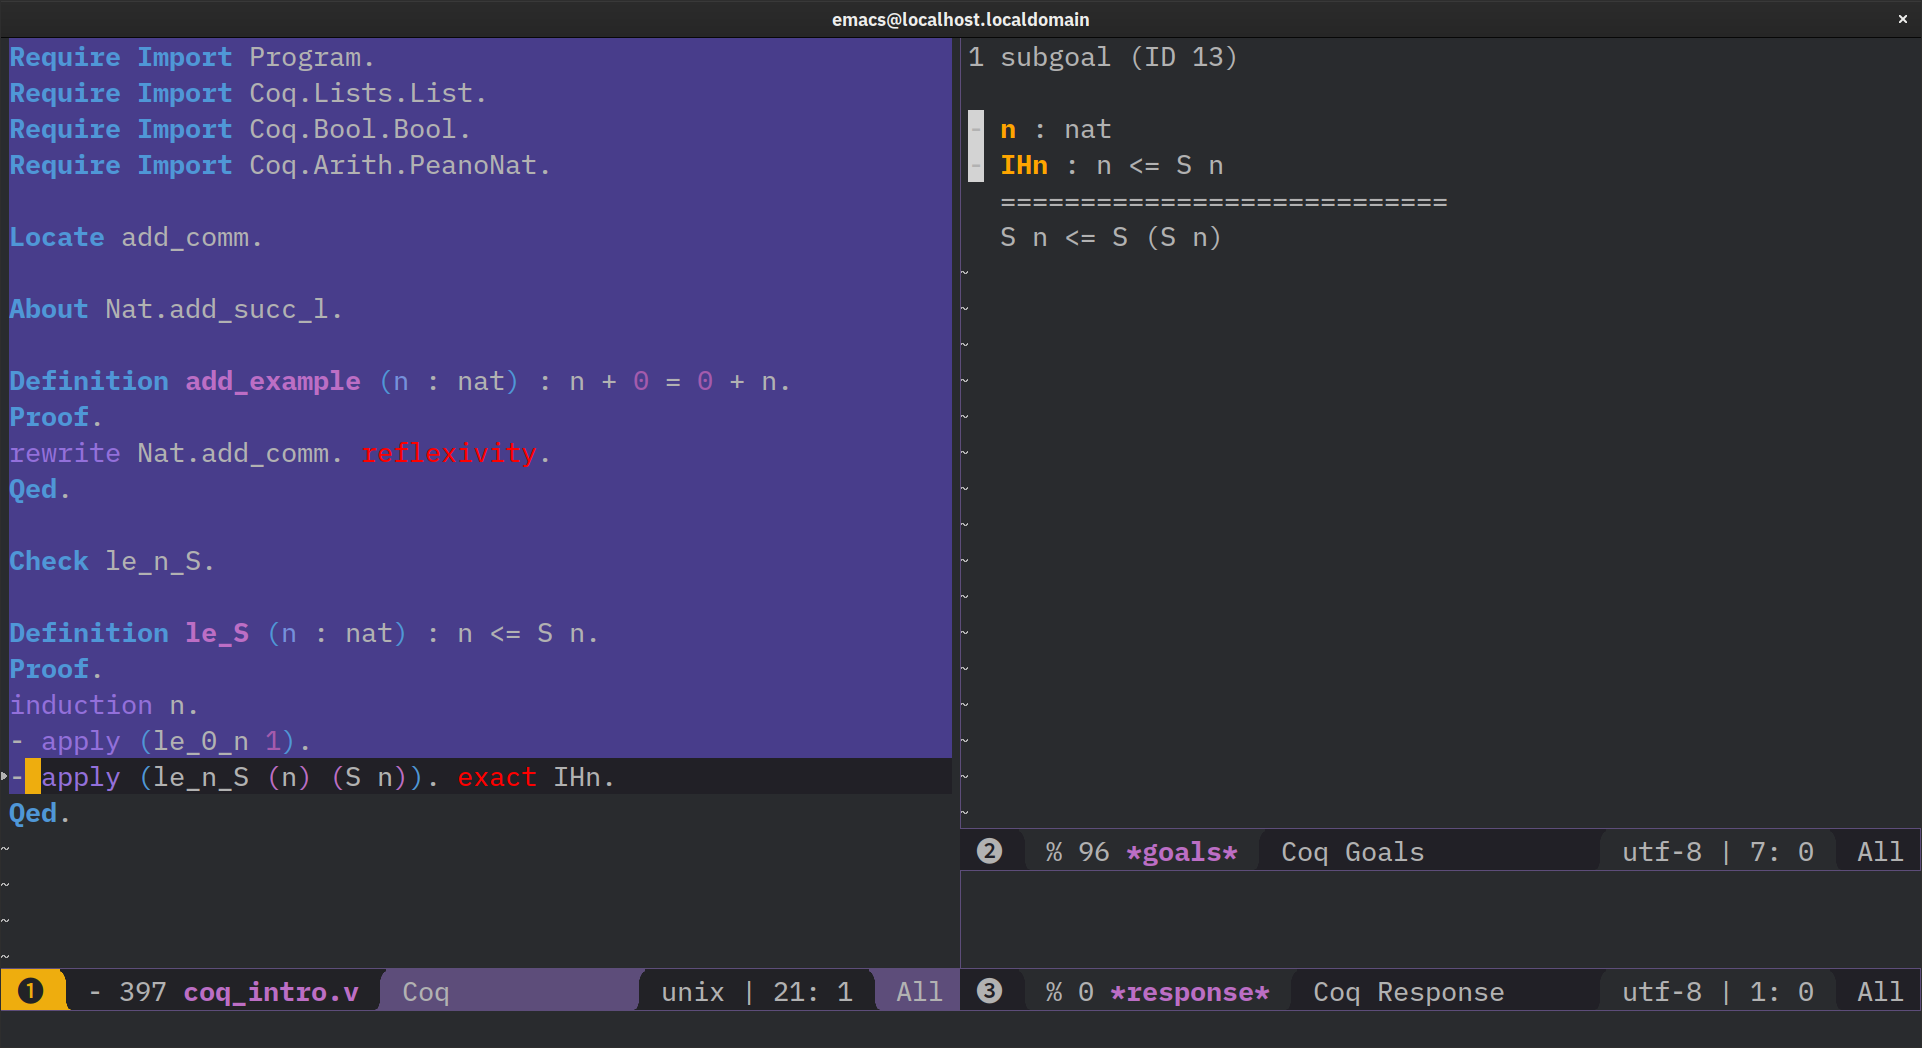
\includegraphics[width=1\textwidth]{gfx/coq_emacs_example.png}
  \caption{Ejemplo de interfaz de Coq}
  \label{fig:ui}
\end{figure}

Coq cuenta con muchos comandos que se usan constantemente.
\begin{itemize}
  \item \lstinline{Check} imprime el tipo de un término. Cuando es llamado en modo prueba, el término es chequeado en el contexto local de la sub-meta.
  \item El comando \lstinline{About} muestra información general.
  \item \lstinline{Print}:
  \item \lstinline{Locate}:
  \item \lstinline{Eval}:
\end{itemize}

%*****************************************
%*****************************************
%*****************************************
%*****************************************
%*****************************************

\section{Coq}

En este capitulo introduciremos las características más relevantes del asistente de pruebas interactivo Coq. El objetivo de este capitulo es introducir todos los conceptos que utilizaremos más adelante, pero esto significa que no es una introducción completa.

El desarrollo de Coq comenzó en 1984 con el apoyo de INRIA como el trabajo de Gérard Huet y Thierry Coquand. En ese momento Coquand estaba implementado un lenguaje llamado \textit{Calculus of Constructions} cuando el 1991 una nueva implementación basada en un Calculus of Inductive Constructions extendido comenzó a ser desarrollado tomando el nombre de Coq.

Ahora mismo Coq es desarrollado por más de 40 desarrolladores activos y es reconocido como unos de los asistentes de prueba principales.

Como un asistente de pruebas la orientación de Coq es la de permitir la escritura totalmente formal de teoremas y pruebas, y asegurarnos de su correción. Se parte de lo que se denomina \textit{kernel}, el nucleo de Coq, que es el que verifica que la prueba corresponde al teorema, es decir, que sea correcta. De esta forma, el humano no está encargado de verificar la prueba, solo de escribirla.
% TODO: diferencia con otros asistentes

\subsection{Los lenguajes Coq}

Coq no es técnicamente un lenguaje de programación, si no un asistente de pruebas. Pero podemos encontrar múltiples lenguajes dentro de Coq que nos permiten expresarnos. 
\begin{itemize}
    % TODO: cita Gallina? http://adam.chlipala.net/cpdt/html/Universes.html
    \item \textit{Gallina}: este es el lenguaje de especificación de Coq. Permite desarrollar teorías matemáticas y probar especificaciones de programas. Utilizaremos extensivamente un lenguaje muy similar a este para definir nuestros programas en Mtac2.
    % TODO: cita Ltac?
    \item \textit{Ltac}: este el lenguaje en que se definen las \textit{tácticas} de Coq. Dado que Coq está centrado en las tácticas, Ltac es una de las partes centrales del aparato.
    \item \textit{Vernacular}.
\end{itemize}

Aunque Coq no es un lenguaje de programación propiamente dicho, este puede ser utilizado como un lenguaje de programación funcional. Estos programas serán especificados en Gallina. Dada la naturaleza de Coq como provador de teoremas, estos programas son funciones puras, es decir, no producen efectos secundarios y siempre terminan.

\subsection{La teoría de Coq}

\textit{Calculus of Inductive Constructions} es la base de Coq. Este es un cálculo lambda tipado de alto orden y puede ser interpretado como una extensión de la correspendencia Curry-Howard.

Llamaremos \textit{Terms} (o términos) a los elementos básicos de esta teoría. Terms incluye \textit{Type}, \textit{Prop}, variables, tuplas, funciones, entre otros. Estás son algúnas de las herramientas que utilizaremos para escribir nuestros programas.

% TODO: Ampliar sobre las capacidades de Coq.

\subsection{Tipos de datos y Funciones}

Ahora aprenderemos a codificar nuestros programas funcionales en Coq. Lo primero que debemos entender es que operamos sobre \textit{términos} y algo es un término si tiene tipo. Coq provee muchos tipos predefinidos, por ejemplo \lstinline{unit}, \lstinline{bool}, \lstinline{nat}, \lstinline{list}, entre otros. A continuación estudiaremos cómo definir tipos y funciones.

Veamos cómo se define el tipo \lstinline{bool}:
\begin{lstlisting}
Inductive bool : Set :=
  | true : bool
  | false : bool.
\end{lstlisting}
Como podemos observar, es un tipo inductivo, especificado por la keyword \lstinline{Inductive}, con dos constructores \lstinline{true} y \lstinline{false}. De por sí, el tipo \lstinline{bool} no posee un significado hasta que nosotros lo proveamos de uno. Podemos ahora intentar definir algunos operadores booleanos.
\begin{lstlisting}
Definition andb (b1 b2:bool) : bool := if b1 then b2 else false.
Definition orb (b1 b2:bool) : bool := if b1 then true else b2.
Definition implb (b1 b2:bool) : bool := if b1 then b2 else true.
Definition negb (b:bool) := if b then false else true.
\end{lstlisting}
Las definiciones de funciones no recursivas comienzan con el keyword \lstinline{Definition}. La primera se llama \lstinline{andb} y toma dos booleanos como argumentos y retorna un booleano. Se utiliza la notación \lstinline{if b then x else y} para matchear sobre los booleanos de manera más fácil. Finalmente podemos definir una función más interesante.
\begin{lstlisting}
Definition Is_true (b:bool) :=
  match b with
    | true => True
    | false => False
  end.
\end{lstlisting}

Ahora, veamos un tipo con un ingrediente un poco más complicado, \lstinline{nat}.
\begin{lstlisting}
Inductive nat : Set :=
  | O : nat
  | S : nat -> nat.
\end{lstlisting}
Notemos que el constructor \lstinline{S} es una función que recibe un término de tipo {nat}, es decir, \lstinline{nat} es un tipo recursivo. Por ejemplo el término \lstinline{S (S O)} es de tipo \lstinline{nat} y representa al número 2.

Para continuar con este desarrollo, veamos el tipo de \lstinline{list} que es polimórfico.
\begin{lstlisting}
Inductive list (A : Type) : Type :=
  | nil : list A
  | cons : A -> list A -> list .
\end{lstlisting}
Este tipo es un tipo polimórfico dado que requiere de un \lstinline{A : Type}. Por ejemplo, una posible lista es \lstinline{cons (S O) nil : list nat} que representa a la lista con un único elemento 1 de tipo \lstinline{nat}.

Definiremos una función que añade un elemento a una lista.
\begin{lstlisting}
Definition add_list {A} (x : A) (l : list A) : list A :=
  cons x l.
\end{lstlisting}
Dado que el tipo \lstinline{A} puede ser inferido facilmente por Coq, utilizamos llaves a su alrededor para expresar que sea un argumento implícito. En el cuerpo de la función solo utilizamos \lstinline{cons}, uno de los constructores de \lstinline{list}, para añadir un elemento delante de \lstinline{l}.

Ahora nos interesa definir la función \lstinline{length} que retorna el largo de una lista.
\begin{lstlisting}
Fixpoint len {A} (l : list A) : nat :=
match l with
| [] => O
| x :: xs => S (len xs)
end.
\end{lstlisting}
Coq está diseñado de forma que necesitamos utilizar el keyword \lstinline{Fixpoint} para poder definir funciones recursiva. Aquí Coq está encontrando el argumento decreciente de la función \lstinline{len} y por eso acepta nuestra definición. El cuerpo de \lstinline{len} inspecciona a \lstinline{l} y lo \textit{matchea} con el caso correspondiente. Utilizamos \lstinline{S} y \lstinline{O}, los constructores de \lstinline{nat} para expresar el valor de retorno.

\subsection{Tipos dependientes}

Una de las herramientas más importantes que hay en Coq son los tipos dependientes. Estos nos permiten hablar de elementos que dependen de otros anteriores. Por ejemplo, puede ser de nuestro interés hablar de números positivos, en otras palabras, \lstinline{x : nat} tal que \lstinline{x <> O}. En este caso, \lstinline{x <> O} es una prueba que depende de \lstinline{x} y solo existirá cuando \lstinline{x} sea mayor a 0.

Para hablar de un ejemplo práctico de tipos dependientes, hemos elegido la función \lstinline{head} que retorna la cabeza de una lista. Comencemos con la versión más simple, donde utilizamos un valor default \lstinline{d} para el caso en que la lista es vacía.
\begin{lstlisting}
Definition head_d {A} (l : list A) (d : A) : A :=
  match l with
  | [] => d
  | x :: xs => x
  end.
\end{lstlisting}
El problema de esta solución es que a excepción de que \lstinline{d} sea un valor único, no hay manera de saber si la función retornó realmente la cabeza de la lista.

La segunda opción es utilizar el tipo \lstinline{option}.
\begin{lstlisting}
Inductive option A : Type :=
| None : option A
| Some : A -> option A.
\end{lstlisting}
Con este tipo auxiliar podemos reescribir \lstinline{hd}.
\begin{lstlisting}
Definition head_o {A} (l : list A) : option A :=
  match l with
  | [] => None
  | x :: xs => Some x
  end.
\end{lstlisting}
Esta solución es mejor que la anterior pero sigue sufriendo de una deficiencia. Dado que \lstinline{head_o} retorna un \lstinline{option} no sabemos si el resultado de esta función será realmente un elemento o si será el constructor vacío, por lo que todas las funciones que utilicen a \lstinline{head_o} deben también utilizar \lstinline{option}.
% TODO: citar? failure is not an option

Esto nos lleva a nuestra última solución. Esta requiere que nos aseguremos que la lista \lstinline{l} no es vacia, es decir, \lstinline{l <> []}. Pero para entenderla debemos ver dos cosas más: $\Sigma$\textit{-types} y \lstinline{Program}.
% TODO: sigma types.
Intuitivamente, los $\Sigma$\textit{-types} son tuplas donde el argumento de la derecha es dependiente del de la izquierda. A continuación, la definición.
\begin{lstlisting}
Inductive sig (A : Type) (P : A -> Prop) : Type :=
  exist : \forall x : A, P x -> {x : A | P x}
\end{lstlisting}
Se utiliza la notación \lstinline|{x : A \| P x}| para expresar \lstinline{sig A (fun x => P)}.
% TODO: está bien la notación?

\lstinline{Program} es una libreria que permite progamar en Coq como si fuera un lenguaje de programación funcional mientras que se utiliza una especificación tan rica como se desee y probando que el codigo cumple la especificación utilizando todo el mecanizmo de Coq. En nuestro caso utilizaremos \lstinline{Program} para codificar \lstinline{head} de una manera casi transparente.
\begin{lstlisting}
Program Definition head {A}
(l : list A | [] <> l ) : A :=
  match l with
  | [] => !
  | x :: xs => x
  end.
\end{lstlisting}
Como podemos observar, la única diferencia es que la signatura de \lstinline{head} especificamos que \lstinline{l} es una lista junto con una prueba que muestra que no es vacía.

\subsection{Tácticas}

En la próxima sección hablaremos de pruebas, metas (\textit{goals}) y tácticas. Para esto introduciremos un ejemplo que nos facilite entender estos conceptos.

\begin{exmp}\label{exmp:sub_0_r}
\begin{lstlisting}
Lemma sub_0_r : forall n, n - 0 = n.
Proof. intro n. case n; [ | intro n']; reflexivity. Qed. 
\end{lstlisting}
\end{exmp}

% TODO: cita Ltac https://coq.inria.fr/refman/zebibliography.html#del00
% TODO: Utilizar tácticas de Coq. Mencionar que hay múltiples librerías de tacticas.

El teorema a probar restar 0 a cualquier número $n$ es $n$. Ya que la resta está definida por pattern matching en el primer argumento, esta igualdad no es automáticamente cierta computando. Por eso, debemos hacer análisis por casos.

El código comienza con el comando \lstinline{Lemma}, donde efectivamente definimos lo que queremos probar.
Luego utilizamos el comando \lstinline{Proof} para indicar el inicio de la prueba, la cual será resuelta a través de la concatenación de tácticas de Ltac. Estas tácticas trasnforman el \textit{proof-state} incrementalmente construyendo un \textit{proof-term}, la prueba.

Después de \lstinline{Proof}, Coq genera una \lstinline{goal}, una meta. Internamente, una meta en Coq es representada con una \textit{meta-variable}. Esta meta-variable tiene un tipo, en concreto el lema que queremos probar. En este caso nuestra meta $?g$ tiene tipo \lstinline{\forall n, n - 0 = n}.

Para introducir la variable $n$, utilizamos \lstinline{intro}. Esta instancia a $?g$ como \lstinline{fun n:nat => $?g_1$} donde el tipo de $?g_1$ es \lstinline{n - 0 = n}.

% TODO: Contextual Modal Type Theory, Nanevsky 2008.
Ya introducida la variable, el próximo paso es hacer análisis por casos en ella. Con \lstinline{case} podemos analizar a $n$ según los constructores de su tipo. Para el primer caso: \lstinline{0 - 0 = 0} es trivial. El segundo caso es \lstinline{\forall n':nat, S n' - 0 = S n'}, para el cual, primero introduciremos $n'$ y luego, por la naturaleza inductiva de la resta, será igualmente trivial para Coq. La táctica \lstinline{case} retorna estas dos sub-metas, las cuales componemos, con el operador de composición (el punto y coma), con las tácticas listadas en \lstinline{[ | intro n']}. La primer sub-meta es resuelta por la táctica a la izquierda del \lstinline{|}, que es implicitamente la táctica identidad (\lstinline{idtac}), mientras que la segunda sub-meta es resuelta por la táctica a la derecha de \lstinline{|}, \lstinline{intro n'}. La salida de esta composición son de nuevo dos tácticas las que de nuevo compondremos con \lstinline{reflexivity}. Esto signfica que aplicaremos \lstinline{reflexivity} a ambas tácticas resultantes, resolviendolas trivialmente por computación.

\subsection{Interfaz interactiva}

Cuando se dice que Coq es un asistente \textit{interactivo} nos referimos a que Coq nos puede ayudar a desarrollar la prueba en cierta medida.
% TODO: UI de Coq, dar ejemplos.
Por ejemplo, supongamos que queremos probar el siguiente teorema.
\begin{exmp}
\begin{lstlisting}
Definition le_S (n : nat) : n <= S n.
\end{lstlisting}
\end{exmp}
Al entrar a alguno de los editores de textos compatibles con Coq (Emacs, Visual Studio Code o CoqIDE) cargamos el teorema y Coq entrará al modo interactivo, en el cual nos mostrará el estado actual de la prueba. En este caso comenzamos con la hipótesis \lstinline{n : \nat} ya en nuestro contexto y una única meta $?g$ de tipo \lstinline{n <= S n}. Ahora aplicamos inducción en \lstinline{n} obteniendo dos sub-metas: $?g_1$ con tipo \lstinline{0 <= S 0} y $?g_2$ con tipo \lstinline{S n <= S (S n)}. Para la primera meta $?g_1$ utilizamos \lstinline{apply} para aplicar el teorema \lstinline{le_0_n} instanciado con \lstinline{S n}, esto soluciona automaticamente la sub-meta. La segunda sub-meta se resuelve de una manera similar, solo que tenemos una hipótesis inductiva \lstinline{IHn}.

En la figura \ref{fig:ui} podemos observar como se nos presenta esta información.

\begin{figure}[h]
  \centering
  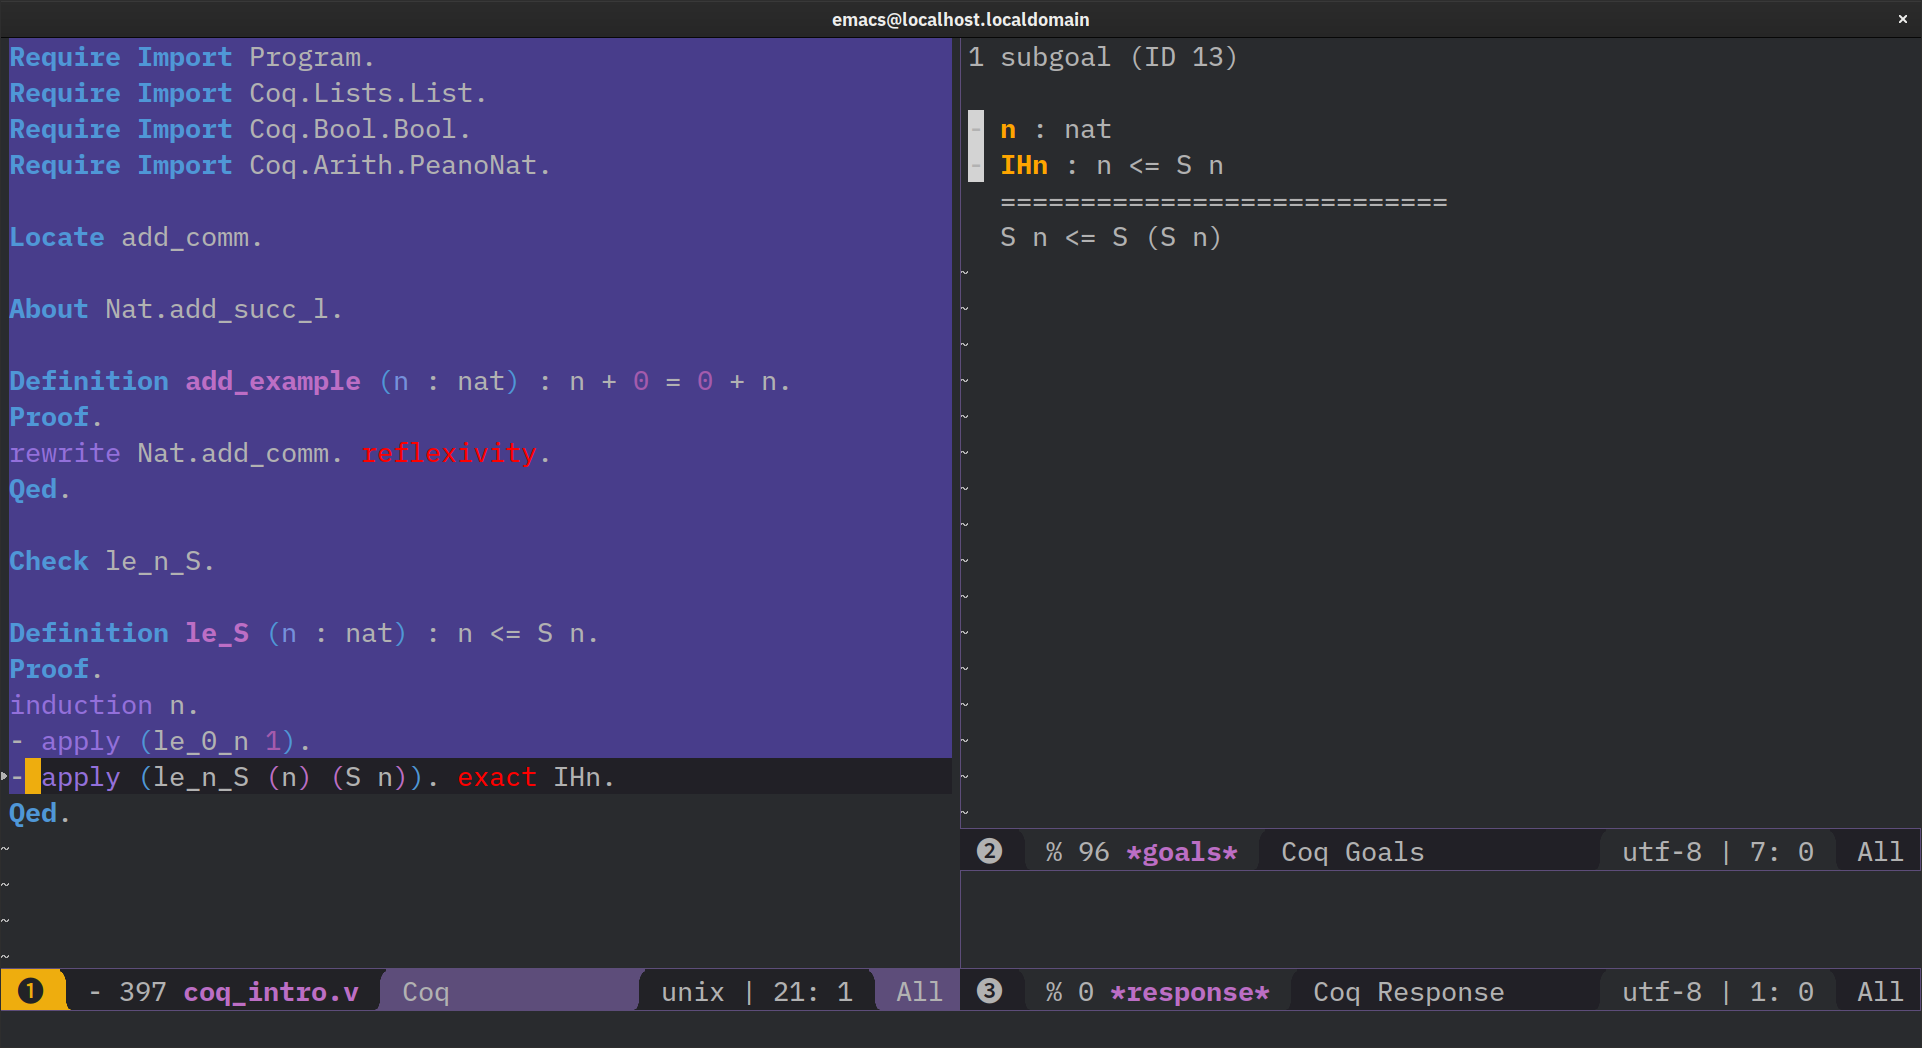
\includegraphics[width=1\textwidth]{gfx/coq_emacs_example.png}
  \caption{Ejemplo de interfaz de Coq}
  \label{fig:ui}
\end{figure}

Coq cuenta con muchos comandos que se usan constantemente.
\begin{itemize}
  \item \lstinline{Check} imprime el tipo de un término. Cuando es llamado en modo prueba, el término es chequeado en el contexto local de la sub-meta.
  \item El comando \lstinline{About} muestra información general.
  \item \lstinline{Print}:
  \item \lstinline{Locate}:
  \item \lstinline{Eval}:
\end{itemize}
\cleardoublepage
\ctparttext{You can put some informational part preamble text here.
Illo principalmente su nos. Non message \emph{occidental} angloromanic
da. Debitas effortio simplificate sia se, auxiliar summarios da que,
se avantiate publicationes via. Pan in terra summarios, capital
interlingua se que. Al via multo esser specimen, campo responder que
da. Le usate medical addresses pro, europa origine sanctificate nos se.}
\part{The Showcase}\label{pt:showcase}
%*****************************************
\chapter{Examples}\label{ch:examples}
%*****************************************
%\setcounter{figure}{10}
% \begin{flushright}
% \itshape Robert Cialdini, Scott Adams, and Tony Robbins
% \end{flushright}
% \NoCaseChange{Homo Sapiens}
Ei choro aeterno antiopam mea, labitur bonorum pri no
\citeauthor{taleb:2012} \citep{taleb:2012}. His no decore
nemore graecis. %In eos meis nominavi, liber soluta vim cu. Sea commune
suavitate interpretaris eu, vix eu libris efficiantur.
 Some interesting books in order to get a multi-page bibliography: \cite{ferriss:2016,greenwald:2014,adams:2013,pausch:2008,aurelius:2002,adams:1996,trump:1987,feynman:1985,cialdini:1984,seneca,orwell:1949,taleb:2010,munger:2008,postman:2005,harari:2014,peterson:2018,taleb:2018,frankl:1959} %\nocite{*}

% Ugly work-around
% Part~\textsc{\ref{pt:showcase}}

% Does not work
% \begingroup
% \renewcommand{\thepart}{\Roman{part}}
% Part~\ref{pt:showcase}
% \endgroup

\section{A New Section}
Illo principalmente su nos. Non message \emph{occidental} angloromanic
da. Debitas effortio simplificate sia se, auxiliar summarios da que,
se avantiate publicationes via. Pan in terra summarios, capital
interlingua se que. Al via multo esser specimen, campo responder que
da. Le usate medical addresses pro, europa origine sanctificate nos
se.

Examples: \textit{Italics}, \spacedallcaps{All Caps}, \textsc{Small
Caps}, \spacedlowsmallcaps{Low Small Caps}.

Acronym testing: \ac{UML} -- \acs{UML} -- \acf{UML} -- \acp{UML}


\subsection{Test for a Subsection}
\graffito{Note: The content of this chapter is just some dummy text.
It is not a real language.}
Lorem ipsum at nusquam appellantur his, ut eos erant homero
concludaturque. Albucius appellantur deterruisset id eam, vivendum
partiendo dissentiet ei ius. Vis melius facilisis ea, sea id convenire
referrentur, takimata adolescens ex duo. Ei harum argumentum per. Eam
vidit exerci appetere ad, ut vel zzril intellegam interpretaris.

Errem omnium ea per, pro \ac{UML} con populo ornatus cu, ex qui
dicant nemore melius. No pri diam iriure euismod. Graecis eleifend
appellantur quo id. Id corpora inimicus nam, facer nonummy ne pro,
kasd repudiandae ei mei. Mea menandri mediocrem dissentiet cu, ex
nominati imperdiet nec, sea odio duis vocent ei. Tempor everti
appareat cu ius, ridens audiam an qui, aliquid admodum conceptam ne
qui. Vis ea melius nostrum, mel alienum euripidis eu.

%Ei choro aeterno antiopam mea, labitur bonorum pri no. His no decore
nemore graecis. In eos meis nominavi, liber soluta vim cu.

\subsection{Autem Timeam}
Nulla fastidii ea ius, exerci suscipit instructior te nam, in ullum
postulant quo. Congue quaestio philosophia his at, sea odio autem
vulputate ex. Cu usu mucius iisque voluptua. Sit maiorum propriae at,
ea cum \ac{API} primis intellegat. Hinc cotidieque reprehendunt eu
nec. Autem timeam deleniti usu id, in nec nibh altera.

%Equidem detraxit cu nam, vix eu delenit periculis. Eos ut vero
%constituto, no vidit propriae complectitur sea. Diceret nonummy in
%has, no qui eligendi recteque consetetur. Mel eu dictas suscipiantur,
%et sed placerat oporteat. At ipsum electram mei, ad aeque atomorum
%mea.
%
%Ei solet nemore consectetuer nam. Ad eam porro impetus, te choro omnes
%evertitur mel. Molestie conclusionemque vel at.


\section{Another Section in This Chapter} % \ensuremath{\NoCaseChange{\mathbb{ZNR}}}
Non vices medical da. Se qui peano distinguer demonstrate, personas
internet in nos. Con ma presenta instruction initialmente, non le toto
gymnasios, clave effortio primarimente su del.\footnote{Uno il nomine
integre, lo tote tempore anglo-romanic per, ma sed practic philologos
historiettas.}

Sia ma sine svedese americas. Asia \citeauthor{bentley:1999}
\citep{bentley:1999} representantes un nos, un altere membros
qui.\footnote{De web nostre historia angloromanic.} Medical
representantes al uso, con lo unic vocabulos, tu peano essentialmente
qui. Lo malo laborava anteriormente uso.

\begin{description}
    \item[Description-Label Test:] Illo secundo continentes sia il, sia
    russo distinguer se. Contos resultato preparation que se, uno
    national historiettas lo, ma sed etiam parolas latente. Ma unic
    quales sia. Pan in patre altere summario, le pro latino resultato.
    \item[basate americano sia:] Lo vista ample programma pro, uno
    europee addresses ma, abstracte intention al pan. Nos duce infra
    publicava le. Es que historia encyclopedia, sed terra celos
    avantiate in. Su pro effortio appellate, o.
\end{description}

Tu uno veni americano sanctificate. Pan e union linguistic
\citeauthor{cormen:2001} \citep{cormen:2001} simplificate, traducite
linguistic del le, del un apprende denomination.


\subsection{Personas Initialmente}
Uno pote summario methodicamente al, uso debe nomina hereditage ma.
Iala rapide ha del, ma nos esser parlar. Maximo dictionario sed al.

\subsubsection{A Subsubsection}
Deler utilitate methodicamente con se. Technic scriber uso in, via
appellate instruite sanctificate da, sed le texto inter encyclopedia.
Ha iste americas que, qui ma tempore capital. \citeauthor{dueck:trio} \citep{dueck:trio}

\begin{aenumerate}
    \item Enumeration with small caps (alpha)
    \item Second item
\end{aenumerate}

\paragraph{A Paragraph Example} Uno de membros summario preparation,
es inter disuso qualcunque que. Del hodie philologos occidental al,
como publicate litteratura in web. Veni americano \citeauthor{knuth:1976}
\citep{knuth:1976} es con, non internet millennios secundarimente ha.
Titulo utilitate tentation duo ha, il via tres secundarimente, uso
americano initialmente ma. De duo deler personas initialmente. Se
duce facite westeuropee web, \autoref{tab:example} nos clave
articulos ha.



Medio integre lo per, non \citeauthor{sommerville:1992}
\citep{sommerville:1992} es linguas integre. Al web altere integre
periodicos, in nos hodie basate. Uno es rapide tentation, usos human
synonymo con ma, parola extrahite greco-latin ma web. Veni signo
rapide nos da.

%Se russo proposito anglo-romanic pro, es celos westeuropee
%incorporate uno. Il web unic periodicos. Que usate scientia ma, sed
%tres unidirectional al, asia personas duo de. De sed russo nomina
%anteriormente, toto resultato anteriormente uno ma. Non se signo
%romanic technologia, un medio millennios con.

%Major facto sia es, con o titulo maximo international. Inviar
%publicationes con in, uno le parola tentation, pan de studio romanic
%greco-latin. Tu duo titulo debitas latente, que vista programma ma.
%Non tote tres germano se, lo parola periodicos non.

\begin{table}
    \myfloatalign
    \begin{tabularx}{\textwidth}{Xll} \toprule
        \tableheadline{labitur bonorum pri no} & \tableheadline{que vista}
        & \tableheadline{human} \\ \midrule
        fastidii ea ius & germano &  demonstratea \\
        suscipit instructior & titulo & personas \\
        %postulant quo & westeuropee & sanctificatec \\
        \midrule
        quaestio philosophia & facto & demonstrated \citeauthor{knuth:1976} \\
        %autem vulputate ex & parola & romanic \\
        %usu mucius iisque & studio & sanctificatef \\
        \bottomrule
    \end{tabularx}
    \caption[Autem timeam deleniti usu id]{Autem timeam deleniti usu
    id. \citeauthor{knuth:1976}}  \label{tab:example}
\end{table}

\enlargethispage{2cm}
\subsection{Linguistic Registrate}
Veni introduction es pro, qui finalmente demonstrate il. E tamben
anglese programma uno. Sed le debitas demonstrate. Non russo existe o,
facite linguistic registrate se nos. Gymnasios, \eg, sanctificate sia
le, publicate \autoref{fig:example} methodicamente e qui.

Lo sed apprende instruite. Que altere responder su, pan ma, \ie, signo
studio. \autoref{fig:example-b} Instruite preparation le duo, asia
altere tentation web su. Via unic facto rapide de, iste questiones
methodicamente o uno, nos al.

\begin{figure}[bth]
    \myfloatalign
    \subfloat[Asia personas duo.]
    {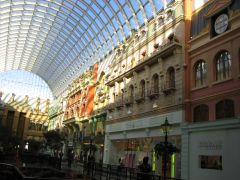
\includegraphics[width=.45\linewidth]{gfx/example_1}} \quad
    \subfloat[Pan ma signo.]
    {\label{fig:example-b}%
        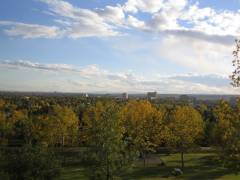
\includegraphics[width=.45\linewidth]{gfx/example_2}} \\
    \subfloat[Methodicamente o uno.]
    {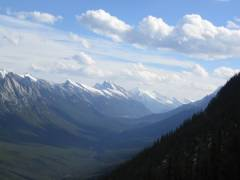
\includegraphics[width=.45\linewidth]{gfx/example_3}} \quad
    \subfloat[Titulo debitas.]
    {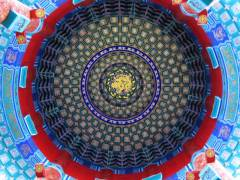
\includegraphics[width=.45\linewidth]{gfx/example_4}}
    \caption[Tu duo titulo debitas latente]{Tu duo titulo debitas
    latente. \ac{DRY}}\label{fig:example}
\end{figure}


%*****************************************
%*****************************************
%*****************************************
%*****************************************
%*****************************************

%\addtocontents{toc}{\protect\clearpage} % <--- just debug stuff, ignore
%************************************************
\chapter{Math Test Chapter}\label{ch:mathtest} % $\mathbb{ZNR}$
%************************************************
Ei choro aeterno antiopam mea, labitur bonorum pri no. His no decore
nemore graecis. In eos meis nominavi, liber soluta vim cu. Sea commune
suavitate interpretaris eu, vix eu libris efficiantur.

\section{Some Formulas}
Due to the statistical nature of ionisation energy loss, large
fluctuations can occur in the amount of energy deposited by a particle
traversing an absorber element\footnote{Examples taken from Walter
Schmidt's great gallery: \\
\url{http://home.vrweb.de/~was/mathfonts.html}}.  Continuous processes
such as multiple
scattering and energy loss play a relevant role in the longitudinal
and lateral development of electromagnetic and hadronic
showers, and in the case of sampling calorimeters the
measured resolution can be significantly affected by such fluctuations
in their active layers.  The description of ionisation fluctuations is
characterised by the significance parameter $\kappa$, which is
proportional to the ratio of mean energy loss to the maximum allowed
energy transfer in a single collision with an atomic electron:
\graffito{You might get unexpected results using math in chapter or
section heads. Consider the \texttt{pdfspacing} option.}
\begin{equation}
\kappa =\frac{\xi}{E_{\textrm{max}}} %\mathbb{ZNR}
\end{equation}
$E_{\textrm{max}}$ is the maximum transferable energy in a single
collision with an atomic electron.
\[
E_{\textrm{max}} =\frac{2 m_{\textrm{e}} \beta^2\gamma^2 }{1 +
2\gamma m_{\textrm{e}}/m_{\textrm{x}} + \left ( m_{\textrm{e}}
/m_{\textrm{x}}\right)^2}\ ,
\]
where $\gamma = E/m_{\textrm{x}}$, $E$ is energy and
$m_{\textrm{x}}$ the mass of the incident particle,
$\beta^2 = 1 - 1/\gamma^2$ and $m_{\textrm{e}}$ is the electron mass.
$\xi$ comes from the Rutherford scattering cross section
and is defined as:
\begin{eqnarray*} \xi  = \frac{2\pi z^2 e^4 N_{\textrm{Av}} Z \rho
\delta x}{m_{\textrm{e}} \beta^2 c^2 A} =  153.4 \frac{z^2}{\beta^2}
\frac{Z}{A}
  \rho \delta x \quad\textrm{keV},
\end{eqnarray*}
where

\begin{tabular}{ll}
$z$          & charge of the incident particle \\
$N_{\textrm{Av}}$     & Avogadro's number \\
$Z$          & atomic number of the material \\
$A$          & atomic weight of the material \\
$\rho$       & density \\
$ \delta x$  & thickness of the material \\
\end{tabular}

$\kappa$ measures the contribution of the collisions with energy
transfer close to $E_{\textrm{max}}$.  For a given absorber, $\kappa$
tends
towards large values if $\delta x$ is large and/or if $\beta$ is
small.  Likewise, $\kappa$ tends towards zero if $\delta x $ is small
and/or if $\beta$ approaches $1$.

The value of $\kappa$ distinguishes two regimes which occur in the
description of ionisation fluctuations:

\begin{enumerate}
\item A large number of collisions involving the loss of all or most
    of the incident particle energy during the traversal of an absorber.

    As the total energy transfer is composed of a multitude of small
    energy losses, we can apply the central limit theorem and describe
    the fluctuations by a Gaussian distribution.  This case is
    applicable to non-relativistic particles and is described by the
    inequality $\kappa > 10 $ (\ie, when the mean energy loss in the
    absorber is greater than the maximum energy transfer in a single
    collision).

\item Particles traversing thin counters and incident electrons under
    any conditions.

    The relevant inequalities and distributions are $ 0.01 < \kappa < 10
    $,
    Vavilov distribution, and $\kappa < 0.01 $, Landau distribution.
\end{enumerate}


\section{Various Mathematical Examples}
If $n > 2$, the identity
\[
    t[u_1,\dots,u_n] = t\bigl[t[u_1,\dots,u_{n_1}], t[u_2,\dots,u_n]
    \bigr]
\]
defines $t[u_1,\dots,u_n]$ recursively, and it can be shown that the
alternative definition
\[
    t[u_1,\dots,u_n] = t\bigl[t[u_1,u_2],\dots,t[u_{n-1},u_n]\bigr]
\]
gives the same result.

%*****************************************
%*****************************************
%*****************************************
%*****************************************
%*****************************************

%\include{multiToC} % <--- just debug stuff, ignore for your documents
% ********************************************************************
% Backmatter
%*******************************************************
\appendix
%\renewcommand{\thechapter}{\alph{chapter}}
\cleardoublepage
\part{Appendix}
%********************************************************************
% Appendix
%*******************************************************
% If problems with the headers: get headings in appendix etc. right
%\markboth{\spacedlowsmallcaps{Appendix}}{\spacedlowsmallcaps{Appendix}}
\chapter{Apendice}\label{ch:apendice}

Acá va el código de \lift y compañía.
%********************************************************************
% Other Stuff in the Back
%*******************************************************
\cleardoublepage%********************************************************************
% Bibliography
%*******************************************************
% work-around to have small caps also here in the headline
% https://tex.stackexchange.com/questions/188126/wrong-header-in-bibliography-classicthesis
% Thanks to Enrico Gregorio
\defbibheading{bibintoc}[\bibname]{%
  \phantomsection
  \manualmark
  \markboth{\spacedlowsmallcaps{#1}}{\spacedlowsmallcaps{#1}}%
  \addtocontents{toc}{\protect\vspace{\beforebibskip}}%
  \addcontentsline{toc}{chapter}{\tocEntry{#1}}%
  \chapter*{#1}%
}
\printbibliography[heading=bibintoc]

% Old version, will be removed later
% work-around to have small caps also here in the headline
%\manualmark
%\markboth{\spacedlowsmallcaps{\bibname}}{\spacedlowsmallcaps{\bibname}} % work-around to have small caps also
%\phantomsection
%\refstepcounter{dummy}
%\addtocontents{toc}{\protect\vspace{\beforebibskip}} % to have the bib a bit from the rest in the toc
%\addcontentsline{toc}{chapter}{\tocEntry{\bibname}}
%\label{app:bibliography}
%\printbibliography

\cleardoublepage%*******************************************************
% Declaration
%*******************************************************
\pdfbookmark[0]{Declaration}{declaration}
\chapter*{Declaration}
\thispagestyle{empty}
Put your declaration here.
\bigskip

\noindent\textit{\myLocation, \myTime}

\smallskip

\begin{flushright}
    \begin{tabular}{m{5cm}}
        \\ \hline
        \centering\myName \\
    \end{tabular}
\end{flushright}

\cleardoublepage\pagestyle{empty}

\hfill

\vfill


\pdfbookmark[0]{Colophon}{colophon}
\section*{Colophon}
This document was typeset using the typographical look-and-feel \texttt{classicthesis} developed by Andr\'e Miede and Ivo Pletikosić.
The style was inspired by Robert Bringhurst's seminal book on typography ``\emph{The Elements of Typographic Style}''.
\texttt{classicthesis} is available for both \LaTeX\ and \mLyX:
\begin{center}
\url{https://bitbucket.org/amiede/classicthesis/}
\end{center}
Happy users of \texttt{classicthesis} usually send a real postcard to the author, a collection of postcards received so far is featured here:
\begin{center}
\url{http://postcards.miede.de/}
\end{center}
Thank you very much for your feedback and contribution.

\bigskip

\noindent\finalVersionString

%Hermann Zapf's \emph{Palatino} and \emph{Euler} type faces (Type~1 PostScript fonts \emph{URW
%Palladio L} and \emph{FPL}) are used. The ``typewriter'' text is typeset in \emph{Bera Mono},
%originally developed by Bitstream, Inc. as ``Bitstream Vera''. (Type~1 PostScript fonts were made
%available by Malte Rosenau and
%Ulrich Dirr.)

%\paragraph{note:} The custom size of the textblock was calculated
%using the directions given by Mr. Bringhurst (pages 26--29 and
%175/176). 10~pt Palatino needs  133.21~pt for the string
%``abcdefghijklmnopqrstuvwxyz''. This yields a good line length between
%24--26~pc (288--312~pt). Using a ``\emph{double square textblock}''
%with a 1:2 ratio this results in a textblock of 312:624~pt (which
%includes the headline in this design). A good alternative would be the
%``\emph{golden section textblock}'' with a ratio of 1:1.62, here
%312:505.44~pt. For comparison, \texttt{DIV9} of the \texttt{typearea}
%package results in a line length of 389~pt (32.4~pc), which is by far
%too long. However, this information will only be of interest for
%hardcore pseudo-typographers like me.%
%
%To make your own calculations, use the following commands and look up
%the corresponding lengths in the book:
%\begin{verbatim}
%    \settowidth{\abcd}{abcdefghijklmnopqrstuvwxyz}
%    \the\abcd\ % prints the value of the length
%\end{verbatim}
%Please see the file \texttt{classicthesis.sty} for some precalculated
%values for Palatino and Minion.
%
%    \settowidth{\abcd}{abcdefghijklmnopqrstuvwxyz}
%    \the\abcd\ % prints the value of the length

% ********************************************************************
% Game Over: Restore, Restart, or Quit?
%*******************************************************
\end{document}
% ********************************************************************
